% !TeX program = xelatex
\PassOptionsToPackage{no-math}{fontspec}
\documentclass[UTF8,11pt,openany,oneside,a4paper,fontset=none]{ctexbook}
\usepackage[a4paper,top=25mm,bottom=25mm,left=26mm,right=26mm,headheight=15pt]{geometry}
\usepackage{fontspec}
\setCJKmainfont{FandolSong-Regular.otf}[BoldFont=FandolSong-Bold.otf,ItalicFont=FandolKai-Regular.otf,Script=Default]
\setCJKsansfont{FandolHei-Regular.otf}[BoldFont=FandolHei-Bold.otf,Script=Default]
\setCJKmonofont{FandolFang-Regular.otf}[Script=Default]
\setmainfont{NimbusRoman-Regular.otf}[Path=fonts/,BoldFont=NimbusRoman-Bold.otf,ItalicFont=NimbusRoman-Italic.otf,BoldItalicFont=NimbusRoman-BoldItalic.otf]
\setsansfont{NimbusSans-Regular.otf}[Path=fonts/,BoldFont=NimbusSans-Bold.otf,ItalicFont=NimbusSans-Italic.otf,BoldItalicFont=NimbusSans-BoldItalic.otf]
\setmonofont{Latin Modern Mono}[Scale=MatchLowercase]
\usepackage{amsmath,amssymb,mathtools,bm}
\usepackage{graphicx,array,booktabs,longtable,multirow}
\usepackage{enumitem,caption,float,needspace}
\usepackage[breakable]{tcolorbox}
\usepackage{fancyhdr,microtype}
\usepackage{hyperref,bookmark,zref-abspage,zref-user}
\hypersetup{unicode=true,hidelinks,bookmarksnumbered=true,
  pdftitle={非线性最小二乘问题的求解方法},
  pdfauthor={K. Madsen; H. B. Nielsen; O. Tingleff},
  pdfsubject={第二版（2004年4月）中文译本}}
\setlength{\parindent}{2em}
\setlength{\parskip}{0.22em}
\linespread{1.18}
\setlength{\emergencystretch}{1.5em}
\allowdisplaybreaks[2]
\setlist{nosep,leftmargin=2em,topsep=0.4em}
\captionsetup{font=small,labelfont=bf,labelsep=quad}
\pagestyle{fancy}
\fancyhf{}
\fancyhead[L]{\small\nouppercase{\leftmark}}
\fancyhead[R]{\small 非线性最小二乘问题的求解方法}
\fancyfoot[C]{\thepage}
\renewcommand{\headrulewidth}{0.3pt}
\fancypagestyle{plain}{\fancyhf{}\fancyfoot[C]{\thepage}\renewcommand{\headrulewidth}{0pt}}
\ctexset{chapter={format=\Huge\bfseries,beforeskip=18pt,afterskip=30pt},section={format=\Large\bfseries}}
\newcommand{\R}{\mathbb{R}}
\newcommand{\T}{\top}
\providecommand{\norm}[1]{\lVert#1\rVert}
\DeclareMathOperator*{\argmin}{arg\,min}
\newcommand{\sourcepage}[1]{\phantomsection\label{src:#1}\zlabel{srcabs:#1}}
\tcbset{colback=white,colframe=black!50,boxrule=0.4pt,arc=0pt,left=6pt,right=6pt,top=5pt,bottom=5pt,before skip=9pt,after skip=9pt}
\newenvironment{statement}[1]{\par\needspace{5\baselineskip}\begin{tcolorbox}[breakable]\noindent\textbf{#1}\par\nobreak\smallskip\noindent\ignorespaces}{\end{tcolorbox}}
\newenvironment{example}[1]{\par\addvspace{0.8em}\needspace{4\baselineskip}\begin{list}{}{\setlength{\leftmargin}{1em}\setlength{\rightmargin}{0pt}}\item[]\textbf{例 #1}\quad\ignorespaces}{\unskip\nobreak\hfill\ensuremath{\blacksquare}\par\end{list}\addvspace{0.5em}}
\newenvironment{algorithmbox}[2]{\par\needspace{7\baselineskip}\begin{tcolorbox}[breakable]\noindent\textbf{算法 #1\quad #2}\par\nobreak\smallskip\begingroup\small}{\par\endgroup\end{tcolorbox}}
\begin{document}
\frontmatter
\pagenumbering{gobble}
\hypersetup{pageanchor=false}
\thispagestyle{empty}
\pdfbookmark[0]{翻译说明}{translation-note}
\begin{center}\vspace*{22mm}{\LARGE\bfseries 翻译说明}\end{center}
\vspace{12mm}
本译本依据 K. Madsen、H. B. Nielsen 与 O. Tingleff 合著的
\textit{Methods for Non-Linear Least Squares Problems} 第二版（2004 年 4 月）英文 PDF 翻译。
\par
译文按原著的章节、段落及定义、定理、例题、算法顺序编排。数学公式采用可编辑的 LaTeX 源码，保留原著编号；图形保留原版矢量线条，图题及自然语言说明译为中文。专有名称、代码标识符和参考文献保留必要的英文。
\par
中文重新排版后页码与英文原版不同。正文及索引中的书内页码引用指向本译本相应内容；参考文献中的出版页码仍按原著列出。原著自身的图号缺口及疑似数学误植照录，并在单独的检查报告中说明。
\par
本页为翻译说明。后续封面、目录、正文、附录、参考文献和索引均对应原著内容。
\clearpage
\begin{titlepage}
\pdfbookmark[0]{封面}{cover}
\centering
{\large IMM\par}
\vspace*{35mm}
{\Huge\bfseries 非线性最小二乘问题\\[8mm]的求解方法\par}
\vspace{15mm}
{\Large 第二版，2004 年 4 月\par}
\vspace{24mm}
{\large K. Madsen\quad H. B. Nielsen\quad O. Tingleff\par}
\vfill
{\large 信息学与数学建模系\\[3mm]丹麦技术大学\par}
\vspace{20mm}
\end{titlepage}
\pagenumbering{roman}
\hypersetup{pageanchor=true}
\pdfbookmark[0]{目录}{contents}
\tableofcontents
\mainmatter
\chapter{引言与定义}
% 原书印刷页 1–4；按源页逐段重译，所有数学均为原生 LaTeX。
\sourcepage{1}
本讲义讨论如下问题。

\begin{statement}{定义 1.1\quad 最小二乘问题}
求 $\mathbf{x}^{*}$，使其为下列函数的一个局部极小点\footnotemark[1]：
\[
 F(\mathbf{x})=\frac12\sum_{i=1}^{m}\bigl(f_i(\mathbf{x})\bigr)^2,
\]
其中 $f_i:\R^n\to\R$，$i=1,\ldots,m$ 是给定的函数，且 $m\ge n$。
\end{statement}
\footnotetext[1]{定义 $F(\mathbf{x})$ 时引入的因子 $\tfrac12$ 不影响 $\mathbf{x}^{*}$。引入它是为了方便，见第~\pageref{src:18}~页。}
\setcounter{footnote}{1}

\begin{example}{1.1}
最小二乘问题的一个重要来源是数据拟合。例如，考虑下图所示的数据点 $(t_1,y_1),\allowbreak\ldots,\allowbreak(t_m,y_m)$。

\begin{figure}[H]
\centering
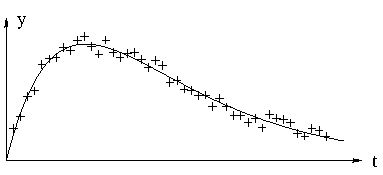
\includegraphics[width=0.67\linewidth]{assets/figures/fig-1-1.pdf}
\setcounter{figure}{0}
\caption{数据点 $\{(t_i,y_i)\}$（以 $+$ 标记）与模型 $M(\mathbf{x},t)$（以实线表示）。}
\label{fig:1.1}
\end{figure}
此外，给定一个拟合模型，
\[
 M(\mathbf{x},t)=x_3e^{x_1t}+x_4e^{x_2t}.
\]

\sourcepage{2}
该模型取决于参数 $\mathbf{x}=[x_1,x_2,x_3,x_4]^{\T}$。我们假定存在某个 $\mathbf{x}^{\dagger}$，使得
\[
 y_i=M(\mathbf{x}^{\dagger},t_i)+\varepsilon_i,
\]
其中 $\{\varepsilon_i\}$ 是数据纵坐标的（测量）误差，假定其表现如同“白噪声”。

对于任意选定的 $\mathbf{x}$，我们都可以计算残差
\[
\begin{aligned}
 f_i(\mathbf{x})&=y_i-M(\mathbf{x},t_i)\\
 &=y_i-x_3e^{x_1t_i}-x_4e^{x_2t_i},\qquad i=1,\ldots,m.
\end{aligned}
\]
对于最小二乘拟合，参数取为残差平方和的极小点 $\mathbf{x}^{*}$。可见，这是定义 1.1 所述形式的问题，其中 $n=4$。图~\ref{fig:1.1} 中的实线表示 $M(\mathbf{x}^{*},t)$ 的图像。
\end{example}

最小二乘问题是以下更一般问题的一种特殊形式：给定函数 $F:\R^n\to\R$，求使这个所谓的目标函数或代价函数取得最小值的自变量。

\begin{statement}{定义 1.2\quad 全局极小点}
给定 $F:\R^n\to\R$。求
\[
 \mathbf{x}^{+}=\operatorname*{arg\,min}_{\mathbf{x}}\{F(\mathbf{x})\}.
\]
\end{statement}

一般而言，这个问题很难求解。我们只介绍求解一个较简单问题的方法，即寻找 $F$ 的局部极小点：在某个区域内使 $F$ 取得最小值的自变量向量，该区域的大小由 $\delta$ 给定，其中 $\delta$ 是一个较小的正数。

\begin{statement}{定义 1.3\quad 局部极小点}
给定 $F:\R^n\to\R$。求 $\mathbf{x}^{*}$，使得
\[
 F(\mathbf{x}^{*})\le F(\mathbf{x})\qquad\text{当 }\norm{\mathbf{x}-\mathbf{x}^{*}}<\delta.
\]
\end{statement}

本章余下部分将讨论优化中的一些基本概念；第 2 章简要回顾为一般代价函数寻找局部极小点的方法。
\sourcepage{3}
更多细节参见 Frandsen 等（2004）。第 3 章给出专为最小二乘问题设计的方法。

我们假定代价函数 $F$ 可微，并且足够光滑，使以下泰勒展开成立\footnote{除非另有说明，$\norm{\cdot}$ 表示 2-范数，即 $\norm{\mathbf{h}}=\sqrt{h_1^2+\cdots+h_n^2}$。}：
\begin{equation}
 F(\mathbf{x}+\mathbf{h})=F(\mathbf{x})+\mathbf{h}^{\T}\mathbf{g}
 +\frac12\mathbf{h}^{\T}\mathbf{H}\mathbf{h}+O(\norm{\mathbf{h}}^3),
 \tag{1.4a}\label{eq:1.4a}
\end{equation}
其中 $\mathbf{g}$ 为梯度，
\begin{equation}
 \mathbf{g}\equiv \mathbf{F}'(\mathbf{x})=
 \begin{bmatrix}
  \dfrac{\partial F}{\partial x_1}(\mathbf{x})\\[1ex]
  \vdots\\[1ex]
  \dfrac{\partial F}{\partial x_n}(\mathbf{x})
 \end{bmatrix},
 \tag{1.4b}\label{eq:1.4b}
\end{equation}
而 $\mathbf{H}$ 为海森矩阵，
\begin{equation}
 \mathbf{H}\equiv \mathbf{F}''(\mathbf{x})=
 \left[\frac{\partial^2F}{\partial x_i\partial x_j}(\mathbf{x})\right].
 \tag{1.4c}\label{eq:1.4c}
\end{equation}

如果 $\mathbf{x}^{*}$ 是局部极小点，且 $\norm{\mathbf{h}}$ 足够小，那么就不可能找到一个点 $\mathbf{x}^{*}+\mathbf{h}$，使其 $F$ 值更小。将这一观察与式~\eqref{eq:1.4a} 结合，得到

\begin{statement}{定理 1.5\quad 局部极小点的必要条件}
如果 $\mathbf{x}^{*}$ 是局部极小点，则
\[
 \mathbf{g}^{*}\equiv \mathbf{F}'(\mathbf{x}^{*})=\mathbf{0}.
\]
\end{statement}

对于满足这一必要条件的自变量，我们使用一个专门的名称。

\begin{statement}{定义 1.6\quad 驻点}
如果
\[
 \mathbf{g}_{\mathrm{s}}\equiv \mathbf{F}'(\mathbf{x}_{\mathrm{s}})=\mathbf{0},
\]
则称 $\mathbf{x}_{\mathrm{s}}$ 为 $F$ 的一个驻点。
\end{statement}

\sourcepage{4}
因此，局部极小点也是驻点，但局部极大点同样也是驻点。既不是局部极大点、也不是局部极小点的驻点称为鞍点。为了判定一个给定的驻点是否为局部极小点，需要计入泰勒级数~\eqref{eq:1.4a} 中的二阶项。代入 $\mathbf{x}_{\mathrm{s}}$，可得
\begin{equation}
\begin{aligned}
 F(\mathbf{x}_{\mathrm{s}}+\mathbf{h})
 &=F(\mathbf{x}_{\mathrm{s}})+\frac12\mathbf{h}^{\T}\mathbf{H}_{\mathrm{s}}\mathbf{h}
   +O(\norm{\mathbf{h}}^3)\\
 &\hspace{1.5em}\text{其中 }\mathbf{H}_{\mathrm{s}}=\mathbf{F}''(\mathbf{x}_{\mathrm{s}}).
\end{aligned}
\tag{1.7}\label{eq:1.7}
\end{equation}

由海森矩阵的定义~\eqref{eq:1.4c} 可知，任意 $\mathbf{H}$ 都是对称矩阵。如果要求 $\mathbf{H}_{\mathrm{s}}$ 正定，那么它的特征值均大于某个数 $\delta>0$（见附录 A），并且
\[
 \mathbf{h}^{\T}\mathbf{H}_{\mathrm{s}}\mathbf{h}>\delta\norm{\mathbf{h}}^2.
\]
这表明，当 $\norm{\mathbf{h}}$ 足够小时，式~\eqref{eq:1.7} 右侧的第二项将支配第三项。而第二项是正的，因此得到

\begin{statement}{定理 1.8\quad 局部极小点的充分条件}
假设 $\mathbf{x}_{\mathrm{s}}$ 是一个驻点，且 $\mathbf{F}''(\mathbf{x}_{\mathrm{s}})$ 正定。则 $\mathbf{x}_{\mathrm{s}}$ 是一个局部极小点。
\end{statement}

如果 $\mathbf{H}_{\mathrm{s}}$ 负定，则 $\mathbf{x}_{\mathrm{s}}$ 是局部极大点。如果 $\mathbf{H}_{\mathrm{s}}$ 不定（即同时具有正特征值和负特征值），则 $\mathbf{x}_{\mathrm{s}}$ 是鞍点。

\chapter{下降法}
% 第2章：原书印刷页5--16，按原文逐页重译；公式及算法均为可编辑原生内容。
\sourcepage{5}
所有非线性优化方法都是迭代方法：从起始点 $\mathbf{x}_0$ 出发，方法产生一列向量
$\mathbf{x}_1,\mathbf{x}_2,\ldots$，它们（希望能够）收敛到给定函数的一个局部极小点
$\mathbf{x}^{\ast}$，见定义~1.3。大多数方法都采取措施，强制满足\emph{下降条件}
\begin{equation}
  F(\mathbf{x}_{k+1})<F(\mathbf{x}_k).
  \tag{2.1}\label{eq:2.1}
\end{equation}
这可以防止迭代收敛到极大点，也降低了收敛到鞍点的可能性。如果给定函数有多个极小点，
结果就取决于起始点 $\mathbf{x}_0$。我们不知道会找到其中的哪一个；它不一定是离
$\mathbf{x}_0$ 最近的极小点。

在许多情况下，方法产生的向量经过两个明显不同的阶段收敛到极小点。当 $\mathbf{x}_0$
远离解时，我们希望方法产生的迭代点稳步向 $\mathbf{x}^{\ast}$ 移动。在迭代的这一
“全局阶段”，只要除了最初几步以外误差不再增大，我们就可以满意，即
\[
  \norm{\mathbf{e}_{k+1}}<\norm{\mathbf{e}_k}\qquad\text{当 }k>K,
\]
其中 $\mathbf{e}_k$ 表示当前误差，
\begin{equation}
  \mathbf{e}_k=\mathbf{x}_k-\mathbf{x}^{\ast}.
  \tag{2.2}\label{eq:2.2}
\end{equation}

在迭代的最后阶段，$\mathbf{x}_k$ 已接近 $\mathbf{x}^{\ast}$，我们希望收敛得更快。
我们区分以下几种情形：

\emph{线性收敛：}
\begin{equation}
  \norm{\mathbf{e}_{k+1}}\leq a\norm{\mathbf{e}_k}
  \qquad\text{当 }\norm{\mathbf{e}_k}\text{ 较小时；}\quad 0<a<1,
  \tag{2.3a}\label{eq:2.3a}
\end{equation}

\sourcepage{6}
\emph{二次收敛：}
\begin{equation}
  \norm{\mathbf{e}_{k+1}}=O\bigl(\norm{\mathbf{e}_k}^{2}\bigr)
  \qquad\text{当 }\norm{\mathbf{e}_k}\text{ 较小时},
  \tag{2.3b}\label{eq:2.3b}
\end{equation}

\emph{超线性收敛：}
\begin{equation}
  \norm{\mathbf{e}_{k+1}}/\norm{\mathbf{e}_k}\longrightarrow0
  \qquad\text{当 }k\longrightarrow\infty.
  \tag{2.3c}\label{eq:2.3c}
\end{equation}

本讲义介绍的方法都是下降法，在每一步迭代中都满足下降条件~(2.1)。从当前迭代点
出发的一步包括：
\begin{enumerate}[label=\arabic*.,leftmargin=2em]
  \item 找到一个下降方向 $\mathbf{h}_{\mathrm d}$（下文讨论）；
  \item 找到一个步长，使 $F$ 值有较大的下降。
\end{enumerate}
因此，下降法的轮廓如下。

\needspace{16\baselineskip}
\begin{algorithmbox}{2.4}{下降法}
\begin{tabbing}
\hspace{1.3em}\=\hspace{1.3em}\=\hspace{1.3em}\=\hspace{1.3em}\=\kill
\textbf{begin}\\
\> $k:=0;\quad\mathbf{x}:=\mathbf{x}_0;\quad\mathit{found}:=\mathrm{false}$
   \quad\{起始点\}\\
\> \textbf{while} $(\textbf{not }\mathit{found})\ \textbf{and}\ (k<k_{\max})$\\
\>\> $\mathbf{h}_{\mathrm d}:=\text{搜索方向}(\mathbf{x})$
   \quad\{从 $\mathbf{x}$ 出发，沿下降方向\}\\
\>\> \textbf{if} （不存在这样的 $\mathbf{h}$）\\
\>\>\> $\mathit{found}:=\mathrm{true}$\quad\{$\mathbf{x}$ 是驻点\}\\
\>\> \textbf{else}\\
\>\>\> $\alpha:=\text{步长}(\mathbf{x},\mathbf{h}_{\mathrm d})$
   \quad\{从 $\mathbf{x}$ 出发，沿 $\mathbf{h}_{\mathrm d}$ 方向\}\\
\>\>\> $\mathbf{x}:=\mathbf{x}+\alpha\mathbf{h}_{\mathrm d};\quad k:=k+1$
   \quad\{下一个迭代点\}\\
\textbf{end}
\end{tabbing}
\end{algorithmbox}

考虑 $F$ 值沿着从 $\mathbf{x}$ 出发、方向为 $\mathbf{h}$ 的射线如何变化。由泰勒展开式~(1.4a)
可知
\begin{equation}
\begin{aligned}
  F(\mathbf{x}+\alpha\mathbf{h})
    &=F(\mathbf{x})+\alpha\mathbf{h}^{\T}\mathbf{F}'(\mathbf{x})+O(\alpha^2)\\
    &\simeq F(\mathbf{x})+\alpha\mathbf{h}^{\T}\mathbf{F}'(\mathbf{x})
       \qquad\text{当 }\alpha\text{ 充分小时}.
\end{aligned}
\tag{2.5}\label{eq:2.5}
\end{equation}
如果 $F(\mathbf{x}+\alpha\mathbf{h})$ 在 $\alpha=0$ 处是关于 $\alpha$ 的减函数，我们就说
$\mathbf{h}$ 是下降方向。这给出如下定义。

\sourcepage{7}
\begin{statement}{定义 2.6\quad 下降方向}
若 $\mathbf{h}^{\T}\mathbf{F}'(\mathbf{x})<0$，则称 $\mathbf{h}$ 是 $F$ 在 $\mathbf{x}$ 处的下降方向。
\end{statement}

如果不存在这样的 $\mathbf{h}$，则 $\mathbf{F}'(\mathbf{x})=\mathbf{0}$，说明此时 $\mathbf{x}$ 是驻点。
否则，我们必须选择 $\alpha$，即确定从 $\mathbf{x}$ 出发沿 $\mathbf{h}_{\mathrm d}$ 所给方向
应走多远，才能使目标函数值下降。一种做法是求出下式的解（或其近似解）：
\begin{equation}
  \alpha_{\mathrm e}=\operatorname*{argmin}_{\alpha>0}
       \{F(\mathbf{x}+\alpha\mathbf{h})\}.
  \tag{2.7}\label{eq:2.7}
\end{equation}
这一过程称为\emph{线搜索}，将在第~2.3~节中讨论。不过，首先介绍两种计算下降方向的方法。

\section{最速下降法}
由~(2.5) 可知，沿 $\alpha\mathbf{h}$ 迈出一步且 $\alpha>0$ 时，函数值的相对下降量满足
\[
  \lim_{\alpha\to0}
  \frac{F(\mathbf{x})-F(\mathbf{x}+\alpha\mathbf{h})}{\alpha\norm{\mathbf{h}}}
  =-\frac{1}{\norm{\mathbf{h}}}\mathbf{h}^{\T}\mathbf{F}'(\mathbf{x})
  =-\norm{\mathbf{F}'(\mathbf{x})}\cos\theta,
\]
其中 $\theta$ 是向量 $\mathbf{h}$ 与 $\mathbf{F}'(\mathbf{x})$ 之间的夹角。这表明，当 $\theta=\pi$，
即采用下式给出的最速下降方向 $\mathbf{h}_{\mathrm{sd}}$ 时，下降率最大：
\begin{equation}
  \mathbf{h}_{\mathrm{sd}}=-\mathbf{F}'(\mathbf{x}).
  \tag{2.8}\label{eq:2.8}
\end{equation}

基于~(2.8) 的方法（即在算法~2.4~中令 $\mathbf{h}_{\mathrm d}=\mathbf{h}_{\mathrm{sd}}$）
称为\emph{最速下降法}或\emph{梯度法}。这一下降方向的选择在局部意义下是“最好的”，
我们可以将它与精确线搜索~(2.7) 结合。这样的方法会收敛，但最后的收敛是线性的，而且往往很慢。
Frandsen 等（2004）的例子表明，在有限计算精度下，即使采用精确线搜索，最速下降法也可能
找不到一个二次多项式的极小点。不过，对于许多问题，这种方法在迭代过程的初始阶段表现相当好。

\sourcepage{8}
这样的考虑引出了所谓的\emph{混合法}。顾名思义，它们基于两种不同的方法：一种在初始阶段
表现好，例如梯度法；另一种在最后阶段表现好，例如下一节介绍的牛顿法。混合法的一个主要
问题是，如何建立在适当时机切换这两种方法的机制。

\section{牛顿法}
我们可以从 $\mathbf{x}^{\ast}$ 是驻点这一条件推导出此方法。根据定义~1.6，它满足
$\mathbf{F}'(\mathbf{x}^{\ast})=\mathbf{0}$。这是一个非线性方程组，由泰勒展开
\[
\begin{aligned}
  \mathbf{F}'(\mathbf{x}+\mathbf{h})
    &=\mathbf{F}'(\mathbf{x})+\mathbf{F}''(\mathbf{x})\mathbf{h}+O\bigl(\norm{\mathbf{h}}^2\bigr)\\
    &\simeq \mathbf{F}'(\mathbf{x})+\mathbf{F}''(\mathbf{x})\mathbf{h}
       \qquad\text{当 }\norm{\mathbf{h}}\text{ 充分小时},
\end{aligned}
\]
可导出\emph{牛顿法}：求解
\begin{equation}
  \mathbf{H}\mathbf{h}_{\mathrm n}=-\mathbf{F}'(\mathbf{x})
  \qquad\text{其中 }\mathbf{H}=\mathbf{F}''(\mathbf{x}),
  \tag{2.9a}\label{eq:2.9a}
\end{equation}
得到 $\mathbf{h}_{\mathrm n}$，并由下式计算下一个迭代点：
\begin{equation}
  \mathbf{x}:=\mathbf{x}+\mathbf{h}_{\mathrm n}.
  \tag{2.9b}\label{eq:2.9b}
\end{equation}

假设 $\mathbf{H}$ 正定，则它非奇异（这意味着~(2.9a) 有唯一解），并且对于所有非零向量
$\mathbf{u}$，都有 $\mathbf{u}^{\T}\mathbf{H}\mathbf{u}>0$。因此，在~(2.9a) 的两边左乘
$\mathbf{h}_{\mathrm n}^{\T}$，得到
\begin{equation}
  0<\mathbf{h}_{\mathrm n}^{\T}\mathbf{H}\mathbf{h}_{\mathrm n}
    =-\mathbf{h}_{\mathrm n}^{\T}\mathbf{F}'(\mathbf{x}),
  \tag{2.10}\label{eq:2.10}
\end{equation}
这说明 $\mathbf{h}_{\mathrm n}$ 是下降方向：它满足定义~2.6~中的条件。

牛顿法在迭代的最后阶段，即 $\mathbf{x}$ 接近 $\mathbf{x}^{\ast}$ 时表现很好。可以证明
（见 Frandsen 等（2004）），如果解处的海森矩阵正定（即定理~1.8~的充分条件成立），
而且当前点位于 $\mathbf{x}^{\ast}$ 周围 $\mathbf{F}''(\mathbf{x})$ 正定的区域内，
\sourcepage{9}
那么就有二次收敛（定义见~(2.3)）。另一方面，如果 $\mathbf{x}$ 位于一个 $\mathbf{F}''(\mathbf{x})$
处处负定且包含驻点的区域内，那么基本牛顿法~(2.9) 将（二次地）收敛到这个驻点，
而该点是一个极大点。要求所迈出的每一步都沿下降方向，可以避免这种情况。

我们可以构造一种基于牛顿法和最速下降法的混合法。根据~(2.10)，如果 $\mathbf{F}''(\mathbf{x})$
正定，牛顿步就保证沿下降方向。因此，这种混合算法的核心部分可概述为
\begin{equation}
\begin{aligned}
  &\textbf{if}\quad \mathbf{F}''(\mathbf{x})\text{ 正定}\\
  &\qquad \mathbf{h}:=\mathbf{h}_{\mathrm n}\\
  &\textbf{else}\\
  &\qquad \mathbf{h}:=\mathbf{h}_{\mathrm{sd}}\\
  &\mathbf{x}:=\mathbf{x}+\alpha\mathbf{h}
\end{aligned}
\tag{2.11}\label{eq:2.11}
\end{equation}
这里，$\mathbf{h}_{\mathrm{sd}}$ 是最速下降方向，$\alpha$ 由线搜索得到，见第~2.3~节。
检验矩阵是否正定的一个好工具是 Cholesky 方法（见附录~A）；检验成功时，该方法还可用来
求解相应的线性方程组。因此，正定性检验几乎不需要额外代价。

第~2.4~节将介绍一些同时计算搜索方向 $\mathbf{h}_{\mathrm d}$ 和步长 $\alpha$ 的方法，
并给出一个不使用线搜索的~(2.11) 版本。这样的混合法可能非常高效，但几乎从未被使用。
原因是它们需要实现 $\mathbf{F}''(\mathbf{x})$ 的计算，而在复杂的应用问题中往往无法做到这一点。
作为替代，可以采用所谓的\emph{拟牛顿法}，它基于一系列逐渐逼近
$\mathbf{H}^{\ast}=\mathbf{F}''(\mathbf{x}^{\ast})$ 的矩阵。第~3.4~节将介绍这样一种方法，另见
Frandsen 等（2004）第~5~章。

\section{线搜索}
给定一点 $\mathbf{x}$ 和一个下降方向 $\mathbf{h}$。下一步迭代是从 $\mathbf{x}$ 沿 $\mathbf{h}$
方向移动。为确定应移动多远，我们研究给定函数沿从 $\mathbf{x}$ 出发、方向为 $\mathbf{h}$
的射线如何变化，
\sourcepage{10}
\begin{equation}
  \varphi(\alpha)=F(\mathbf{x}+\alpha\mathbf{h}),
  \qquad\mathbf{x}\text{ 和 }\mathbf{h}\text{ 固定},\quad\alpha\geq0.
  \tag{2.12}\label{eq:2.12}
\end{equation}
图~2.1~给出了 $\varphi(\alpha)$ 变化情况的一个例子。

\begin{figure}[H]
\centering
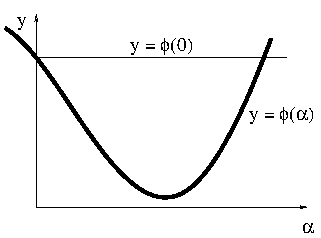
\includegraphics[width=0.53\linewidth]{assets/figures/fig-2-1.pdf}
\setcounter{figure}{0}
\caption{目标函数沿搜索直线的变化。}\label{fig:2.1}
\end{figure}

由于 $\mathbf{h}$ 是下降方向，故有
\[
  \varphi'(0)=\mathbf{h}^{\T}\mathbf{F}'(\mathbf{x})<0,
\]
这表明，如果 $\alpha$ 充分小，就能满足下降条件~(2.1)，它等价于
\[
  \varphi(\alpha)<\varphi(0).
\]
通常会给定一个 $\alpha$ 的初始猜测值，例如牛顿法中的 $\alpha=1$。
图~2.1~说明可能出现三种不同的情况：
\begin{enumerate}[label=\arabic*$^{\circ}$,leftmargin=2.4em]
  \item $\alpha$ 很小，因而目标函数值的下降量很小。应增大 $\alpha$。
  \item $\alpha$ 太大：$\varphi(\alpha)\geq\varphi(0)$。应减小 $\alpha$，
        以满足下降条件~(2.1)。
  \item $\alpha$ 接近 $\varphi(\alpha)$ 的极小点\footnote{更准确地说，是 $\varphi$
        的第一个局部极小点。如果把 $\alpha$ 增大到图~2.1~所示区间之外，完全有可能
        接近 $F$ 的另一个局部极小点。}。接受这一 $\alpha$ 值。
\end{enumerate}

\sourcepage{11}
\emph{精确线搜索}是一个产生序列 $\alpha_1,\alpha_2,\ldots$ 的迭代过程。
其目的是找到~(2.7) 所定义的真正极小点 $\alpha_{\mathrm e}$，当迭代值
$\alpha_{\mathrm s}$ 满足
\[
  |\varphi'(\alpha_{\mathrm s})|\leq\tau\,|\varphi'(0)|
\]
时，算法停止，其中 $\tau$ 是一个较小的正数。迭代中，可以根据已计算的值
\[
  \varphi(\alpha_k)=F(\mathbf{x}+\alpha_k\mathbf{h})
  \qquad\text{和}\qquad
  \varphi'(\alpha_k)=\mathbf{h}^{\T}\mathbf{F}'(\mathbf{x}+\alpha_k\mathbf{h})
\]
来近似 $\varphi(\alpha)$ 的变化。详见 Frandsen 等（2004）第~2.5--2.6~节。

精确线搜索可能浪费很多计算时间：当 $\mathbf{x}$ 远离 $\mathbf{x}^{\ast}$ 时，搜索方向
$\mathbf{h}$ 可能与 $\mathbf{x}^{\ast}-\mathbf{x}$ 的方向相差甚远，没有必要非常精确地找到
$\varphi$ 的真正极小值。这就是所谓的\emph{非精确线搜索}的出发点：只要一个
$\alpha$ 值不属于上面列出的第~$1^{\circ}$ 或第~$2^{\circ}$ 种情况，就可以接受它。
我们采用比下降条件~(2.1) 更严格的条件，即
\begin{equation}
  \varphi(\alpha_{\mathrm s})
  \leq\varphi(0)+\gamma_1\cdot\varphi'(0)\cdot\alpha
  \qquad\text{其中 }0<\gamma_1<1.
  \tag{2.13a}\label{eq:2.13a}
\end{equation}
这保证了不会出现第~$2^{\circ}$ 种情况。第~$1^{\circ}$ 种情况对应于点
$(\alpha,\varphi(\alpha))$ 太接近起点处的切线，因此再补充条件
\begin{equation}
  \varphi'(\alpha_{\mathrm s})\geq\gamma_2\cdot\varphi'(0)
  \qquad\text{其中 }\gamma_1<\gamma_2<1.
  \tag{2.13b}\label{eq:2.13b}
\end{equation}
如果 $\alpha$ 的初始猜测值满足这两个准则，我们就接受它作为 $\alpha_{\mathrm s}$。
否则，必须按照前述精确线搜索的方式迭代。详见 Frandsen 等（2004）第~2.5~节。

\section{信赖域法与阻尼法}
假设有一个模型 $L$，描述 $F$ 在当前迭代点 $\mathbf{x}$ 邻域内的性质，
\begin{equation}
  F(\mathbf{x}+\mathbf{h})\simeq L(\mathbf{h})
  \equiv F(\mathbf{x})+\mathbf{h}^{\T}\mathbf{c}
       +\tfrac12\mathbf{h}^{\T}\mathbf{B}\mathbf{h},
  \tag{2.14}\label{eq:2.14}
\end{equation}

\sourcepage{12}
其中 $\mathbf{c}\in\R^n$，矩阵 $\mathbf{B}\in\R^{n\times n}$ 是对称的。本节的基本思想
可以推广到其他形式的模型，但本讲义只需要~(2.14) 所给形式的 $L$。通常，这一模型是
$F$ 在 $\mathbf{x}$ 附近的二阶泰勒展开，例如~(1.4a) 右端的前三项；$L(\mathbf{h})$ 也可以是
这一展开的近似。一般而言，只有 $\mathbf{h}$ 充分小时，这样的模型才是好的近似。

下面介绍两种在确定步子 $\mathbf{h}$ 时考虑这一点的方法。所得步子沿下降方向，并可在
算法~2.4~中取 $\alpha=1$ 使用。

在\emph{信赖域法}中，我们假设已知一个正数 $\Delta$，使模型在以 $\mathbf{x}$ 为中心、
半径为 $\Delta$ 的球内足够准确，并按下式确定步子：
\begin{equation}
  \mathbf{h}=\mathbf{h}_{\mathrm{tr}}
  \equiv\operatorname*{argmin}_{\norm{\mathbf{h}}\leq\Delta}\{L(\mathbf{h})\}.
  \tag{2.15}\label{eq:2.15}
\end{equation}

在\emph{阻尼法}中，步子由下式确定：
\begin{equation}
  \mathbf{h}=\mathbf{h}_{\mathrm{dm}}
  \equiv\operatorname*{argmin}_{\mathbf{h}}
  \{L(\mathbf{h})+\tfrac12\mu\mathbf{h}^{\T}\mathbf{h}\},
  \tag{2.16}\label{eq:2.16}
\end{equation}
其中\emph{阻尼参数} $\mu\geq0$。可以看出，附加项
$\tfrac12\mu\mathbf{h}^{\T}\mathbf{h}=\tfrac12\mu\norm{\mathbf{h}}^2$ 对较大的步子施加惩罚。

基于上述任一方法，算法~2.4~的核心部分都具有如下形式：
\begin{equation}
\begin{aligned}
  &\text{由~(2.15) 或~(2.16) 计算 }\mathbf{h}\\
  &\textbf{if}\quad F(\mathbf{x}+\mathbf{h})<F(\mathbf{x})\\
  &\qquad\mathbf{x}:=\mathbf{x}+\mathbf{h}\\
  &\text{更新 }\Delta\text{ 或 }\mu
\end{aligned}
\tag{2.17}\label{eq:2.17}
\end{equation}
若步子 $\mathbf{h}$ 满足下降条件~(2.1)，这就相当于 $\alpha=1$。否则，$\alpha=0$，
即不移动\footnote{这两类方法也有包含真正线搜索的版本：寻找 $F$ 值更小的点
$\mathbf{x}+\alpha\mathbf{h}$，并利用线搜索中获得的信息更新 $\Delta$ 或 $\mu$。
对于许多问题，这类版本采用的迭代步数较少，但累计函数求值次数更多。}。
不过，我们不会停滞在
\sourcepage{13}
$\mathbf{x}$ 处（除非 $\mathbf{x}=\mathbf{x}^{\ast}$）：通过适当地修改 $\Delta$ 或 $\mu$，
我们力求在下一次迭代中得到更好的结果。

由于假定 $\mathbf{h}$ 充分小时 $L(\mathbf{h})$ 是 $F(\mathbf{x}+\mathbf{h})$ 的良好近似，
所以一步失败的原因是 $\mathbf{h}$ 太大，应当缩小。另外，如果这一步被接受，那么从新的
迭代点出发也许可以采用更大的步子，从而减少到达 $\mathbf{x}^{\ast}$ 所需的步数。

对于已经计算出的步子，可以用所谓的\emph{增益比}来评价模型的质量，
\begin{equation}
  \varrho=\frac{F(\mathbf{x})-F(\mathbf{x}+\mathbf{h})}{L(\mathbf{0})-L(\mathbf{h})},
  \tag{2.18}\label{eq:2.18}
\end{equation}
即函数值的实际下降量与预测下降量之比。按构造，分母为正；如果这一步没有沿下降方向移动，
分子为负，此时步子太大，应当缩小。

在信赖域法中，我们通过半径 $\Delta$ 的大小来控制步长。下面的更新策略被广泛采用：
\begin{equation}
\begin{aligned}
  &\textbf{if}\quad\varrho<0.25\\
  &\qquad\Delta:=\Delta/2\\
  &\textbf{elseif}\quad\varrho>0.75\\
  &\qquad\Delta:=\max\{\Delta,3*\norm{\mathbf{h}}\}
\end{aligned}
\tag{2.19}\label{eq:2.19}
\end{equation}
因此，如果 $\varrho<\tfrac14$，就决定采用较小的步子；而 $\varrho>\tfrac34$
则表明可能可以采用更大的步子。信赖域算法对阈值 $0.25$ 和 $0.75$、除数 $p_1=2$
或乘数 $p_2=3$ 的小幅改变并不敏感，但必须恰当地选择 $p_1$ 和 $p_2$，使
$\Delta$ 值不会发生振荡。

在阻尼法中，较小的 $\varrho$ 值表明应增大阻尼因子，从而加重对大步子的惩罚。
较大的 $\varrho$ 值则表明，对于计算出的 $\mathbf{h}$，$L(\mathbf{h})$ 是
$F(\mathbf{x}+\mathbf{h})$ 的良好近似，此时可减小阻尼。下面这个与~(2.19) 类似的策略
被广泛使用，它最初由 Marquardt（1963）提出，

\sourcepage{14}
\begin{equation}
\begin{aligned}
  &\textbf{if}\quad\varrho<0.25\\
  &\qquad\mu:=\mu*2\\
  &\textbf{elseif}\quad\varrho>0.75\\
  &\qquad\mu:=\mu/3
\end{aligned}
\tag{2.20}\label{eq:2.20}
\end{equation}
同样，方法对阈值 $0.25$、$0.75$ 或数值 $p_1=2$、$p_2=3$ 的小幅改变并不敏感，
但必须恰当地选择 $p_1$ 和 $p_2$，使 $\mu$ 值不会发生振荡。经验表明，跨越阈值
$0.25$ 和 $0.75$ 时的不连续变化可能引起“抖动”（第~\pageref{src:27}~页的
例~3.7~对此有说明），从而减慢收敛。我们在 Nielsen（1999）中证明，以下策略的表现
通常优于~(2.20)：
\begin{equation}
\begin{aligned}
  &\textbf{if}\quad\varrho>0\\
  &\qquad\mu:=\mu*\max\{\tfrac13,1-(2\varrho-1)^3\};\quad\nu:=2\\
  &\textbf{else}\\
  &\qquad\mu:=\mu*\nu;\quad\nu:=2*\nu
\end{aligned}
\tag{2.21}\label{eq:2.21}
\end{equation}
因子 $\nu$ 初始化为 $\nu=2$。注意，连续多次失败会使 $\mu$ 值迅速增大。
图~2.2~展示了这两个更新公式。

\begin{figure}[H]
\centering
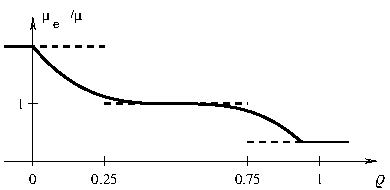
\includegraphics[width=0.64\linewidth]{assets/figures/fig-2-2.pdf}
\setcounter{figure}{1}
\caption{按~(2.21) 且取 $\nu=2$ 更新 $\mu$（实线），以及 Marquardt 的策略~(2.20)（虚线）。}
\label{fig:2.2}
\end{figure}

\subsection{迭代步的计算}
在阻尼法中，步子通过求函数
\[
  \psi_{\mu}(\mathbf{h})=L(\mathbf{h})+\tfrac12\mu\mathbf{h}^{\T}\mathbf{h}
\]
的驻点来计算。

\sourcepage{15}
这意味着 $\mathbf{h}_{\mathrm{dm}}$ 是方程
\[
  \psi'_{\mu}(\mathbf{h})=\mathbf{L}'(\mathbf{h})+\mu\mathbf{h}=\mathbf{0}
\]
的一个解。由~(2.14) 中 $L(\mathbf{h})$ 的定义可知，这等价于
\begin{equation}
  (\mathbf{B}+\mu\mathbf{I})\mathbf{h}_{\mathrm{dm}}=-\mathbf{c},
  \tag{2.22}\label{eq:2.22}
\end{equation}
其中 $\mathbf{I}$ 为单位矩阵。如果 $\mu$ 充分大，对称矩阵 $\mathbf{B}+\mu\mathbf{I}$ 就是
正定的（附录~A~中有证明），于是由定理~1.8~可知 $\mathbf{h}_{\mathrm{dm}}$ 是 $L$ 的极小点。

\begin{example}{2.1}
在\emph{阻尼牛顿法}中，模型 $L(\mathbf{h})$ 由 $\mathbf{c}=\mathbf{F}'(\mathbf{x})$ 和
$\mathbf{B}=\mathbf{F}''(\mathbf{x})$ 给出，因而~(2.22) 化为
\[
  \bigl(\mathbf{F}''(\mathbf{x})+\mu\mathbf{I}\bigr)\mathbf{h}_{\mathrm{dn}}=-\mathbf{F}'(\mathbf{x}).
\]
$\mathbf{h}_{\mathrm{dn}}$ 称为阻尼牛顿步。如果 $\mu$ 很大，则
\[
  \mathbf{h}_{\mathrm{dn}}\simeq-\frac{1}{\mu}\mathbf{F}'(\mathbf{x}),
\]
即沿接近最速下降方向的方向迈出一小步。另一方面，如果 $\mu$ 很小，
$\mathbf{h}_{\mathrm{dn}}$ 就接近牛顿步 $\mathbf{h}_{\mathrm n}$。因此，可以把阻尼牛顿法
看作最速下降法与牛顿法的混合。
\end{example}

我们将在第~3.2~节重新讨论阻尼法。

在信赖域法中，步子 $\mathbf{h}_{\mathrm{tr}}$ 是一个\emph{约束优化问题}的解，
\begin{equation}
\begin{aligned}
  &\text{最小化}\quad L(\mathbf{h})\\
  &\text{约束条件}\quad\mathbf{h}^{\T}\mathbf{h}\leq\Delta^2.
\end{aligned}
\tag{2.23}\label{eq:2.23}
\end{equation}
详细讨论这个问题超出了本讲义的范围（见 Madsen 等（2004），或 Nocedal 与
Wright（1999）第~4.1~节）。这里只提及它的几个性质。

如果~(2.14) 中的矩阵 $\mathbf{B}$ 正定，那么 $L$ 的无约束极小点是方程
\sourcepage{16}
\[
  \mathbf{B}\mathbf{h}=-\mathbf{c}
\]
的解；如果这个解足够小（即满足 $\mathbf{h}^{\T}\mathbf{h}\leq\Delta^2$），它就是所需的步子
$\mathbf{h}_{\mathrm{tr}}$。否则，约束是有效的，问题也更复杂。与第~\pageref{src:11}~页
所用论证类似，可以看出，我们不必计算~(2.23) 的真正解；第~3.3~节和第~3.4~节将介绍
两种计算 $\mathbf{h}_{\mathrm{tr}}$ 近似值的方法。

最后，在 $\mathbf{B}$ 正定的情形下，介绍阻尼法与信赖域法的两个相似之处。
当无约束极小点位于信赖域之外时，可以证明（Madsen 等（2004）的定理~2.11），
存在一个 $\lambda>0$，使得
\begin{equation}
  \mathbf{B}\mathbf{h}_{\mathrm{tr}}+\mathbf{c}=-\lambda\mathbf{h}_{\mathrm{tr}}.
  \tag{2.24a}\label{eq:2.24a}
\end{equation}
将这个方程移项，再与~(2.22) 比较，可见 $\mathbf{h}_{\mathrm{tr}}$ 与采用阻尼参数
$\mu=\lambda$ 算出的阻尼步 $\mathbf{h}_{\mathrm{dm}}$ 完全相同。另一方面，也可以证明
（Frandsen 等（2004）的定理~5.11），如果给定 $\mu\geq0$ 并计算出
$\mathbf{h}_{\mathrm{dm}}$，则
\begin{equation}
  \mathbf{h}_{\mathrm{dm}}
  =\operatorname*{argmin}_{\norm{\mathbf{h}}\leq\norm{\mathbf{h}_{\mathrm{dm}}}}
      \{L(\mathbf{h})\},
  \tag{2.24b}\label{eq:2.24b}
\end{equation}
即 $\mathbf{h}_{\mathrm{dm}}$ 等于信赖域半径 $\Delta=\norm{\mathbf{h}_{\mathrm{dm}}}$
所对应的 $\mathbf{h}_{\mathrm{tr}}$。因此，这两类方法密切相关，但对于给出相同步子的
$\Delta$ 值与 $\mu$ 值，它们之间并不存在简单的联系公式。

\chapter{非线性最小二乘问题}
\sourcepage{17}
在本讲义余下的部分中，我们将讨论非线性最小二乘问题的求解方法。给定向量函数 $\mathbf{f}:\R^n\mapsto\R^m$，其中 $m\geq n$。我们希望使 $\norm{\mathbf{f}(\mathbf{x})}$ 最小，等价地，就是求
\begin{equation}
  \mathbf{x}^*=\operatorname*{arg\,min}_{\mathbf{x}}\{F(\mathbf{x})\},
  \tag{3.1a}\label{eq:3.1a}
\end{equation}
其中
\begin{equation}
  F(\mathbf{x})=\frac12\sum_{i=1}^m\bigl(f_i(\mathbf{x})\bigr)^2
  =\frac12\norm{\mathbf{f}(\mathbf{x})}^2
  =\frac12\mathbf{f}(\mathbf{x})^{\T}\mathbf{f}(\mathbf{x}).
  \tag{3.1b}\label{eq:3.1b}
\end{equation}

最小二乘问题可以用一般的优化方法求解，但我们将介绍效率更高的专门方法。在许多情况下，尽管这些方法不需要实现二阶导数，它们仍能获得优于线性收敛的速度，有时甚至能达到二次收敛。

在描述本章的方法时，我们需要 $F$ 的导数公式。假设 $\mathbf{f}$ 具有连续的二阶偏导数，则其 Taylor 展开可写为
\begin{equation}
  \mathbf{f}(\mathbf{x}+\mathbf{h})=\mathbf{f}(\mathbf{x})+\mathbf{J}(\mathbf{x})\mathbf{h}
  +O(\norm{\mathbf{h}}^2),
  \tag{3.2a}\label{eq:3.2a}
\end{equation}
其中，$\mathbf{J}\in\R^{m\times n}$ 是 Jacobian 矩阵。这个矩阵包含各分量函数的一阶偏导数，
\begin{equation}
  \bigl(\mathbf{J}(\mathbf{x})\bigr)_{ij}
  =\frac{\partial f_i}{\partial x_j}(\mathbf{x}).
  \tag{3.2b}\label{eq:3.2b}
\end{equation}
对于 $F:\R^n\mapsto\R$，由式~\eqref{eq:3.1b} 的第一种写法可得\sourcepage{18}\footnote{如果在定义~\eqref{eq:3.1b} 中没有使用因子 $\tfrac12$，那么许多表达式中都会出现一个令人烦恼的因子 $2$。}
\begin{equation}
  \frac{\partial F}{\partial x_j}(\mathbf{x})
  =\sum_{i=1}^m f_i(\mathbf{x})\frac{\partial f_i}{\partial x_j}(\mathbf{x}).
  \tag{3.3}\label{eq:3.3}
\end{equation}
因此，式~\eqref{eq:1.4b} 中的梯度为
\begin{equation}
  \mathbf{F}'(\mathbf{x})=\mathbf{J}(\mathbf{x})^{\T}\mathbf{f}(\mathbf{x}).
  \tag{3.4a}\label{eq:3.4a}
\end{equation}
我们还需要 $F$ 的 Hessian 矩阵。由式~\eqref{eq:3.3} 可见，其第 $(j,k)$ 个元素为
\[
  \frac{\partial^2 F}{\partial x_j\partial x_k}(\mathbf{x})
  =\sum_{i=1}^m\left(
    \frac{\partial f_i}{\partial x_j}(\mathbf{x})
    \frac{\partial f_i}{\partial x_k}(\mathbf{x})
    +f_i(\mathbf{x})\frac{\partial^2 f_i}{\partial x_j\partial x_k}(\mathbf{x})
  \right),
\]
这表明
\begin{equation}
  \mathbf{F}''(\mathbf{x})=\mathbf{J}(\mathbf{x})^{\T}\mathbf{J}(\mathbf{x})
  +\sum_{i=1}^m f_i(\mathbf{x})f_i''(\mathbf{x}).
  \tag{3.4b}\label{eq:3.4b}
\end{equation}

\begin{example}{3.1}
式~(3.1) 最简单的情形是 $\mathbf{f}(\mathbf{x})$ 具有如下形式：
\[
  \mathbf{f}(\mathbf{x})=\mathbf{b}-\mathbf{A}\mathbf{x},
\]
其中，向量 $\mathbf{b}\in\R^m$ 和矩阵 $\mathbf{A}\in\R^{m\times n}$ 均已给定。我们称之为\emph{线性最小二乘问题}。在这种情况下，对所有 $\mathbf{x}$ 都有 $\mathbf{J}(\mathbf{x})=-\mathbf{A}$，由式~\eqref{eq:3.4a} 可见
\[
  \mathbf{F}'(\mathbf{x})=-\mathbf{A}^{\T}(\mathbf{b}-\mathbf{A}\mathbf{x}).
\]
当 $\mathbf{x}^*$ 为所谓\emph{正规方程}的解时，这个梯度等于零；正规方程为
\begin{equation}
  (\mathbf{A}^{\T}\mathbf{A})\mathbf{x}^*=\mathbf{A}^{\T}\mathbf{b}.
  \tag{3.5}\label{eq:3.5}
\end{equation}
该问题也可写成
\[
  \mathbf{A}\mathbf{x}^*\simeq\mathbf{b},
\]
另一种求解途径是\emph{正交变换}：寻找正交矩阵 $\mathbf{Q}$，使得
\sourcepage{19}
\[
  \mathbf{Q}^{\T}\mathbf{A}=\begin{bmatrix}\mathbf{R}\\\mathbf{0}\end{bmatrix},
\]
其中，$\mathbf{R}\in\R^{n\times n}$ 为上三角矩阵。通过对下列方程组进行回代，即可求得解\footnote{形如 $u_{p:q}$ 的表达式表示由元素 $u_i$（$i=p,\ldots,q$）组成的子向量。矩阵 $\mathbf{A}$ 的第 $i$ 行和第 $j$ 列分别记为 $\mathbf{A}_{i,:}$ 和 $\mathbf{A}_{:,j}$。}：
\[
  \mathbf{R}\mathbf{x}^*=(\mathbf{Q}^{\T}\mathbf{b})_{1:n}.
\]
与通过正规方程求解相比，这种方法更加准确。

在 MATLAB 中，假设数组 \texttt{A} 和 \texttt{b} 分别存放矩阵 $\mathbf{A}$ 和向量 $\mathbf{b}$，则命令 \verb|A\b| 返回通过正交变换算得的最小二乘解。

正如本册的标题所示，我们假设 $\mathbf{f}$ 是非线性的，因此不再详细讨论线性问题。相关内容可参见 Madsen 和 Nielsen（2002）第~2~章，或 Golub 和 Van Loan（1996）第~5.2~节。
\end{example}

\begin{example}{3.2}
在例~1.1 中，我们见到了由数据拟合产生的非线性最小二乘问题。另一个应用是求解非线性方程组，
\[
  \mathbf{f}(\mathbf{x}^*)=\mathbf{0},\qquad\text{其中 }\mathbf{f}:\R^n\mapsto\R^n.
\]
我们可以使用 Newton--Raphson 法：从初始猜测 $\mathbf{x}_0$ 出发，按以下算法计算 $\mathbf{x}_1,\mathbf{x}_2,\ldots$。该算法的依据是寻找使 $\mathbf{f}(\mathbf{x}+\mathbf{h})=\mathbf{0}$ 的 $\mathbf{h}$，并忽略式~\eqref{eq:3.2a} 中的 $O(\norm{\mathbf{h}}^2)$ 项，
\begin{equation}
  \begin{aligned}
    &\text{求解 }\mathbf{J}(\mathbf{x}_k)\mathbf{h}_k=-\mathbf{f}(\mathbf{x}_k)\text{，得到 }\mathbf{h}_k,\\
    &\mathbf{x}_{k+1}=\mathbf{x}_k+\mathbf{h}_k.
  \end{aligned}
  \tag{3.6}\label{eq:3.6}
\end{equation}
这里的 Jacobian 矩阵 $\mathbf{J}$ 由式~\eqref{eq:3.2b} 给出。如果 $\mathbf{J}(\mathbf{x}^*)$ 非奇异，那么该方法在最终阶段具有二次收敛性，即当 $d_k=\norm{\mathbf{x}_k-\mathbf{x}^*}$ 很小时，有 $\norm{\mathbf{x}_{k+1}-\mathbf{x}^*}=O(d_k^2)$。然而，如果 $\mathbf{x}_k$ 远离 $\mathbf{x}^*$，就可能走得更远。

我们可以重新表述该问题，使本章即将介绍的所有“工具”都能派上用场：式~\eqref{eq:3.6} 的一个解，是式~(3.1) 所定义函数 $F$ 的一个全局极小点，
\[
  F(\mathbf{x})=\frac12\norm{\mathbf{f}(\mathbf{x})}^2,
\]
\sourcepage{20}
因为 $F(\mathbf{x}^*)=0$，而当 $\mathbf{f}(\mathbf{x})\ne\mathbf{0}$ 时，$F(\mathbf{x})>0$。例如，可以把式~\eqref{eq:3.6} 中近似解的更新改为
\[
  \mathbf{x}_{k+1}=\mathbf{x}_k+\alpha_k\mathbf{h}_k,
\]
其中，$\alpha_k$ 通过对函数 $\varphi(\alpha)=F(\mathbf{x}_k+\alpha\mathbf{h}_k)$ 作线搜索求得。

作为一个具体的例子，我们考虑取自 Powell（1970）的如下问题：
\[
  \mathbf{f}(\mathbf{x})=\begin{bmatrix}
    x_1\\[2pt]
    \dfrac{10x_1}{x_1+0.1}+2x_2^2
  \end{bmatrix},
\]
它的唯一解为 $\mathbf{x}^*=\mathbf{0}$。其 Jacobian 矩阵为
\[
  \mathbf{J}(\mathbf{x})=\begin{bmatrix}
    1&0\\
    (x_1+0.1)^{-2}&4x_2
  \end{bmatrix},
\]
在解处这个矩阵是奇异的。

若取 $\mathbf{x}_0=[3,\,1]^{\T}$，并在上述算法中采用精确线搜索，则迭代点收敛至 $\mathbf{x}_c\simeq[1.8016,\,0]^{\T}$，它并不是解。另一方面，容易看出，算法~\eqref{eq:3.6} 给出的迭代点为 $\mathbf{x}_k=[0,\,y_k]^{\T}$，其中 $y_{k+1}=\tfrac12 y_k$，也就是说，迭代线性收敛于解。

在后面的若干例子中，我们还将回到这个问题，考察不同方法如何处理它。
\end{example}

\section{Gauss--Newton法}
这种方法是后面几节将要介绍的高效方法的基础。它以向量函数各分量的一阶导数的实现为基础。在特殊情况下，它能像一般优化中的 Newton 法一样达到二次收敛，参见 Frandsen 等（2004）。

Gauss--Newton 法基于 $\mathbf{x}$ 邻域内 $\mathbf{f}$ 各分量的线性近似（即 $\mathbf{f}$ 的线性模型）：当 $\norm{\mathbf{h}}$ 很小时，由 Taylor 展开式~(3.2) 可见
\begin{equation}
  \mathbf{f}(\mathbf{x}+\mathbf{h})\simeq\ell(\mathbf{h})
  \equiv\mathbf{f}(\mathbf{x})+\mathbf{J}(\mathbf{x})\mathbf{h}.
  \tag{3.7a}\label{eq:3.7a}
\end{equation}
将其代入 $F$ 的定义式~(3.1)，可得
\sourcepage{21}
\begin{equation}
  \begin{aligned}
    F(\mathbf{x}+\mathbf{h})&\simeq L(\mathbf{h})
      \equiv\frac12\ell(\mathbf{h})^{\T}\ell(\mathbf{h})\\
    &=\frac12\mathbf{f}^{\T}\mathbf{f}+\mathbf{h}^{\T}\mathbf{J}^{\T}\mathbf{f}
      +\frac12\mathbf{h}^{\T}\mathbf{J}^{\T}\mathbf{J}\mathbf{h}\\
    &=F(\mathbf{x})+\mathbf{h}^{\T}\mathbf{J}^{\T}\mathbf{f}
      +\frac12\mathbf{h}^{\T}\mathbf{J}^{\T}\mathbf{J}\mathbf{h}
  \end{aligned}
  \tag{3.7b}\label{eq:3.7b}
\end{equation}
（其中，$\mathbf{f}=\mathbf{f}(\mathbf{x})$，$\mathbf{J}=\mathbf{J}(\mathbf{x})$）。\emph{Gauss--Newton 步} $\mathbf{h}_{\mathrm{gn}}$ 使 $L(\mathbf{h})$ 最小，
\[
  \mathbf{h}_{\mathrm{gn}}=\operatorname*{arg\,min}_{\mathbf{h}}\{L(\mathbf{h})\}.
\]
容易看出，$L$ 的梯度和 Hessian 矩阵为
\begin{equation}
  \mathbf{L}'(\mathbf{h})=\mathbf{J}^{\T}\mathbf{f}+\mathbf{J}^{\T}\mathbf{J}\mathbf{h},
  \qquad \mathbf{L}''(\mathbf{h})=\mathbf{J}^{\T}\mathbf{J}.
  \tag{3.8}\label{eq:3.8}
\end{equation}
与式~\eqref{eq:3.4a} 比较可知，$\mathbf{L}'(\mathbf{0})=\mathbf{F}'(\mathbf{x})$。此外，矩阵 $\mathbf{L}''(\mathbf{h})$ 与 $\mathbf{h}$ 无关。它是对称矩阵；如果 $\mathbf{J}$ 满秩，即它的列向量线性无关，那么 $\mathbf{L}''(\mathbf{h})$ 还是正定矩阵，参见附录~A。这意味着 $L(\mathbf{h})$ 具有唯一的极小点，可通过求解以下方程得到：
\begin{equation}
  (\mathbf{J}^{\T}\mathbf{J})\mathbf{h}_{\mathrm{gn}}=-\mathbf{J}^{\T}\mathbf{f}.
  \tag{3.9}\label{eq:3.9}
\end{equation}
这是 $F$ 的一个下降方向，因为
\begin{equation}
  \mathbf{h}_{\mathrm{gn}}^{\T}\mathbf{F}'(\mathbf{x})
  =\mathbf{h}_{\mathrm{gn}}^{\T}(\mathbf{J}^{\T}\mathbf{f})
  =-\mathbf{h}_{\mathrm{gn}}^{\T}(\mathbf{J}^{\T}\mathbf{J})\mathbf{h}_{\mathrm{gn}}<0.
  \tag{3.10}\label{eq:3.10}
\end{equation}
因此，可以在算法~2.4 中用 $\mathbf{h}_{\mathrm{gn}}$ 作为 $\mathbf{h}_{\mathrm d}$。其典型迭代步为
\begin{equation}
  \begin{aligned}
    &\text{求解 }(\mathbf{J}^{\T}\mathbf{J})\mathbf{h}_{\mathrm{gn}}=-\mathbf{J}^{\T}\mathbf{f},\\
    &\mathbf{x}:=\mathbf{x}+\alpha\mathbf{h}_{\mathrm{gn}},
  \end{aligned}
  \tag{3.11}\label{eq:3.11}
\end{equation}
其中，$\alpha$ 由线搜索确定。经典的 Gauss--Newton 法在每一步都取 $\alpha=1$。可以证明，带线搜索的方法在满足以下条件时具有收敛保证：
\begin{enumerate}[label=\alph*)]
  \item $\{\mathbf{x}\mid F(\mathbf{x})\leq F(\mathbf{x}_0)\}$ 有界；
  \item 每一步的 Jacobian 矩阵 $\mathbf{J}(\mathbf{x})$ 都满秩。
\end{enumerate}

在第~2~章中，我们看到用于优化的 Newton 法具有二次收敛性。Gauss--Newton 法通常并非如此。
\sourcepage{22}
为看清这一点，我们比较两种方法所用的搜索方向，
\[
  \mathbf{F}''(\mathbf{x})\mathbf{h}_{\mathrm n}=-\mathbf{F}'(\mathbf{x})
  \qquad\text{和}\qquad
  \mathbf{L}''(\mathbf{h})\mathbf{h}_{\mathrm{gn}}=-\mathbf{L}'(\mathbf{0}).
\]
我们在式~\eqref{eq:3.8} 后已经指出，两者的右端相同，但由式~\eqref{eq:3.4b} 和式~\eqref{eq:3.8} 可见，它们的系数矩阵有所不同：
\begin{equation}
  \mathbf{F}''(\mathbf{x})=\mathbf{L}''(\mathbf{h})+\sum_{i=1}^m f_i(\mathbf{x})f_i''(\mathbf{x}).
  \tag{3.12}\label{eq:3.12}
\end{equation}
因此，如果 $\mathbf{f}(\mathbf{x}^*)=\mathbf{0}$，那么当 $\mathbf{x}$ 接近 $\mathbf{x}^*$ 时，就有 $\mathbf{L}''(\mathbf{h})\simeq \mathbf{F}''(\mathbf{x})$，从而 Gauss--Newton 法也能达到二次收敛。如果函数 $\{f_i\}$ 的曲率很小，或者 $\{|f_i(\mathbf{x}^*)|\}$ 很小，则可以期待超线性收敛；但一般情况下，只能期待线性收敛。值得注意的是，$F(\mathbf{x}^*)$ 的值控制着收敛速度。

\begin{example}{3.3}
考虑 $n=1$、$m=2$ 的简单问题，定义为
\[
  \mathbf{f}(x)=\begin{bmatrix}x+1\\\lambda x^2+x-1\end{bmatrix},
  \qquad
  F(x)=\frac12(x+1)^2+\frac12(\lambda x^2+x-1)^2.
\]
于是
\[
  F'(x)=2\lambda^2x^3+3\lambda x^2-2(\lambda-1)x,
\]
所以 $x=0$ 是 $F$ 的一个驻点。又有
\[
  F''(x)=6\lambda^2x^2+6\lambda x-2(\lambda-1).
\]
这说明，如果 $\lambda<1$，则 $F''(0)>0$，因此 $x=0$ 是一个局部极小点；实际上，它是全局极小点。

Jacobian 矩阵为
\[
  \mathbf{J}(x)=\begin{bmatrix}1\\2\lambda x+1\end{bmatrix},
\]
从 $x_k$ 出发，经典 Gauss--Newton 法给出
\[
  x_{k+1}=x_k-
  \frac{2\lambda^2x_k^3+3\lambda x_k^2-2(\lambda-1)x_k}
       {2+4\lambda x_k+4\lambda^2x_k^2}.
\]
现在，如果 $\lambda\ne0$ 且 $x_k$ 接近零，则
\[
  x_{k+1}=x_k+(\lambda-1)x_k+O(x_k^2)
  =\lambda x_k+O(x_k^2).
\]
\sourcepage{23}
因此，当 $|\lambda|<1$ 时，迭代线性收敛。如果 $\lambda<-1$，则经典 Gauss--Newton 法无法找到这个极小点。例如，取 $\lambda=-2$、$x_0=0.1$，迭代点会表现出看似混沌的行为，
\[
  \begin{array}{r|r}
    k&x_k\\\hline
    0&0.1000\\
    1&-0.3029\\
    2&0.1368\\
    3&-0.4680\\
    \vdots&\vdots
  \end{array}
\]
最后，如果 $\lambda=0$，则
\[
  x_{k+1}=x_k-x_k=0,
\]
即只需一步就找到了这个解。这是因为此时 $\mathbf{f}$ 是线性函数。
\end{example}

\begin{example}{3.4}
对于例~1.1 中的数据拟合问题，Jacobian 矩阵的第 $i$ 行为
\[
  \mathbf{J}(\mathbf{x})_{i,:}
  =\begin{bmatrix}
    -x_3t_i e^{x_1t_i}&-x_4t_i e^{x_2t_i}&-e^{x_1t_i}&-e^{x_2t_i}
  \end{bmatrix}.
\]
如果问题是\emph{相容的}（即 $\mathbf{f}(\mathbf{x}^*)=\mathbf{0}$），那么只要 $x_1^*$ 与 $x_2^*$ 有显著差别，带线搜索的 Gauss--Newton 法在最终阶段就具有二次收敛性。如果 $x_1^*=x_2^*$，则 $\operatorname{rank}(\mathbf{J}(\mathbf{x}^*))\leq2$，Gauss--Newton 法就会失效。

如果一个或多个测量误差较大，那么 $\mathbf{f}(\mathbf{x}^*)$ 中会有一些较大的分量，这可能会减慢收敛速度。

在 MATLAB 中，可以用一个十分紧凑的函数来计算 $\mathbf{f}$ 和 $\mathbf{J}$：假设 \texttt{x} 存放当前迭代点，$m\times2$ 数组 \texttt{ty} 存放数据点的坐标。下面的函数返回 \texttt{f} 和 \texttt{J}，其中分别存放 $\mathbf{f}(\mathbf{x})$ 和 $\mathbf{J}(\mathbf{x})$。
\begin{verbatim}
function  [f, J] = fitexp(x, ty)
  t = ty(:,1); y = ty(:,2);
  E = exp(t * [x(1), x(2)]);
  f = y - E*[x(3); x(4)];
  J = -[x(3)*t.*E(:,1), x(4)*t.*E(:,2), E];
\end{verbatim}
\end{example}

% 原书印刷页 24--33。公式与算法均为原生可编辑 LaTeX。
\begin{example}{3.5}
\sourcepage{24}
考虑例~3.2 中的问题：对于 $\mathbf{f}:\R^n\to\R^n$，求解 $\mathbf{f}(\mathbf{x}^*)=\mathbf{0}$。若用 Newton--Raphson 法求解这个问题，其典型迭代步为
\[
  \text{求解 }\mathbf{J}(\mathbf{x})\mathbf{h}_{\mathrm{nr}}=-\mathbf{f}(\mathbf{x});\qquad \mathbf{x}:=\mathbf{x}+\mathbf{h}_{\mathrm{nr}}.
\]
把 Gauss--Newton 法用于极小化 $F(\mathbf{x})=\tfrac12 \mathbf{f}(\mathbf{x})^{\T}\mathbf{f}(\mathbf{x})$ 时，其典型步骤为
\[
  \text{求解 }\bigl(\mathbf{J}(\mathbf{x})^{\T}\mathbf{J}(\mathbf{x})\bigr)\mathbf{h}_{\mathrm{gn}}=-\mathbf{J}(\mathbf{x})^{\T}\mathbf{f}(\mathbf{x});
  \qquad \mathbf{x}:=\mathbf{x}+\mathbf{h}_{\mathrm{gn}}.
\]
注意，$\mathbf{J}(\mathbf{x})$ 是方阵，并且我们假设它非奇异。因此 $(\mathbf{J}(\mathbf{x})^{\T})^{-1}$ 存在，进而有 $\mathbf{h}_{\mathrm{gn}}=\mathbf{h}_{\mathrm{nr}}$。所以，把 Gauss--Newton 法用于例~3.2 中的 Powell 问题时，会遇到该例讨论 Newton--Raphson 法时所遇到的同样困难。
\end{example}

这些例子表明，无论是否采用线搜索，Gauss--Newton 法都有可能失败。不过，在许多应用中它的表现相当好，尽管它通常只有线性收敛性，而实现了二阶导数的 Newton 法具有二次收敛性。

第~3.2 节和第~3.3 节给出两种全局性能更好的方法，第~3.4 节则对第一种方法作一些修改，以获得超线性的最终收敛速度。

\section{Levenberg--Marquardt 法}\label{sec:lm}
Levenberg（1944）以及后来的 Marquardt（1963）提出采用阻尼 Gauss--Newton 法，参见第~2.4 节。步 $\mathbf{h}_{\mathrm{lm}}$ 由式~\eqref{eq:3.9} 的以下修改来定义：
\begin{equation}
  (\mathbf{J}^{\T}\mathbf{J}+\mu \mathbf{I})\mathbf{h}_{\mathrm{lm}}=-\mathbf{g},
  \qquad \mathbf{g}=\mathbf{J}^{\T}\mathbf{f},\quad \mu\geq0.
  \tag{3.13}\label{eq:3.13}
\end{equation}
这里，$\mathbf{J}=\mathbf{J}(\mathbf{x})$，$\mathbf{f}=\mathbf{f}(\mathbf{x})$。阻尼参数 $\mu$ 有以下几方面作用：
\begin{enumerate}[label=\alph*),leftmargin=2.2em]
\item 对所有 $\mu>0$，系数矩阵都是正定的，这保证 $\mathbf{h}_{\mathrm{lm}}$ 是下降方向，参见式~\eqref{eq:3.10}。
\sourcepage{25}
\item 当 $\mu$ 很大时，有
\[
  \mathbf{h}_{\mathrm{lm}}\simeq-\frac1\mu \mathbf{g}=-\frac1\mu \mathbf{F}'(\mathbf{x}),
\]
即沿最速下降方向走一个短步。当当前迭代点离解较远时，这是有益的。
\item 若 $\mu$ 很小，则 $\mathbf{h}_{\mathrm{lm}}\simeq \mathbf{h}_{\mathrm{gn}}$。在迭代的最后阶段，即 $\mathbf{x}$ 接近 $\mathbf{x}^*$ 时，这是一个很好的步。若 $F(\mathbf{x}^*)=0$（或非常小），则可以获得（近乎）二次的最终收敛速度。
\end{enumerate}
因此，阻尼参数既影响步的方向，也影响步的大小，这使我们得以构造一种不需要专门线搜索的方法。

初始 $\mu$ 值的选择应与 $\mathbf{A}_0=\mathbf{J}(\mathbf{x}_0)^{\T}\mathbf{J}(\mathbf{x}_0)$ 中元素的大小有关，例如令
\begin{equation}
  \mu_0=\tau\cdot\max_i\{a_{ii}^{(0)}\},
  \tag{3.14}\label{eq:3.14}
\end{equation}
其中 $\tau$ 由用户选择。\footnote[3]{算法对 $\tau$ 的选择不是很敏感。不过，按照经验，若认为 $\mathbf{x}_0$ 是 $\mathbf{x}^*$ 的良好近似，就应取较小的值，例如 $\tau=10^{-6}$；否则可取 $\tau=10^{-3}$，甚至 $\tau=1$。}迭代过程中可以按第~2.4 节所述更新 $\mu$ 的大小。更新由增益比控制：
\[
  \varrho=\frac{F(\mathbf{x})-F(\mathbf{x}+\mathbf{h}_{\mathrm{lm}})}{L(\mathbf{0})-L(\mathbf{h}_{\mathrm{lm}})},
\]
其中分母是线性模型~\eqref{eq:3.7b} 预测的增益，
\[
\begin{aligned}
 L(\mathbf{0})-L(\mathbf{h}_{\mathrm{lm}})
  &=-\mathbf{h}_{\mathrm{lm}}^{\T}\mathbf{J}^{\T}\mathbf{f}
      -\tfrac12\mathbf{h}_{\mathrm{lm}}^{\T}\mathbf{J}^{\T}\mathbf{J}\mathbf{h}_{\mathrm{lm}}\\
  &=-\tfrac12\mathbf{h}_{\mathrm{lm}}^{\T}
      \bigl(2\mathbf{g}+(\mathbf{J}^{\T}\mathbf{J}+\mu \mathbf{I}-\mu \mathbf{I})\mathbf{h}_{\mathrm{lm}}\bigr)\\
  &=\tfrac12\mathbf{h}_{\mathrm{lm}}^{\T}(\mu \mathbf{h}_{\mathrm{lm}}-\mathbf{g}).
\end{aligned}
\]
注意，$\mathbf{h}_{\mathrm{lm}}^{\T}\mathbf{h}_{\mathrm{lm}}$ 和 $-\mathbf{h}_{\mathrm{lm}}^{\T}\mathbf{g}$ 都为正，因此 $L(\mathbf{0})-L(\mathbf{h}_{\mathrm{lm}})$ 保证为正。

较大的 $\varrho$ 值表示 $L(\mathbf{h}_{\mathrm{lm}})$ 是 $F(\mathbf{x}+\mathbf{h}_{\mathrm{lm}})$ 的良好近似，这时可以减小 $\mu$，使下一个 Levenberg--Marquardt
\sourcepage{26}
步更接近 Gauss--Newton 步。若 $\varrho$ 很小（甚至为负），则 $L(\mathbf{h}_{\mathrm{lm}})$ 是一个较差的近似，应增大 $\mu$，一方面使方向更接近最速下降方向，另一方面缩短步长。有多种方式可以同时达到这两个目的，参见第~\pageref{src:14}~页和下面的例~3.7。

算法的停止准则应体现如下事实：在全局极小点处有 $\mathbf{F}'(\mathbf{x}^*)=\mathbf{g}(\mathbf{x}^*)=\mathbf{0}$。因此可以采用
\begin{equation}
  \norm{\mathbf{g}}_{\infty}\leq\varepsilon_1,
  \tag{3.15a}\label{eq:3.15a}
\end{equation}
其中 $\varepsilon_1$ 是用户选定的一个很小的正数。另一个有用的准则是，当 $\mathbf{x}$ 的变化很小时停止：
\begin{equation}
  \norm{\mathbf{x}_{\mathrm{new}}-\mathbf{x}}\leq\varepsilon_2(\norm{\mathbf{x}}+\varepsilon_2).
  \tag{3.15b}\label{eq:3.15b}
\end{equation}
这个表达式使步长准则从 $\norm{\mathbf{x}}$ 很大时的相对步长 $\varepsilon_2$，平滑过渡到 $\mathbf{x}$ 接近 $\mathbf{0}$ 时的绝对步长 $\varepsilon_2^2$。最后，与所有迭代过程一样，需要设置防止无限循环的保护条件：
\begin{equation}
  k\geq k_{\max}.
  \tag{3.15c}\label{eq:3.15c}
\end{equation}
$\varepsilon_2$ 和 $k_{\max}$ 也由用户选择。

例如，若 $\varepsilon_1$ 取得太小，以至舍入误差的影响很大，最后两个准则就会发挥作用。这种情形通常表现为 $F$ 的实际增益与线性模型~\eqref{eq:3.7b} 预测的增益吻合较差，因而每一步都要增大 $\mu$。采用增大 $\mu$ 的策略~\eqref{eq:2.21}，这时 $\mu$ 会迅速增长，使 $\norm{\mathbf{h}_{\mathrm{lm}}}$ 变得很小，于是过程将由准则~\eqref{eq:3.15b} 停止。

算法概括如下。

% 原版算法为印刷页 27 页首浮动块；此处紧随其引导句，以免割裂例 3.6。
\needspace{24\baselineskip}
\sourcepage{27}
\begin{algorithmbox}{3.16}{Levenberg--Marquardt 法}
\begin{tabbing}
\hspace{1.2em}\=\hspace{1.2em}\=\hspace{1.2em}\=\hspace{1.2em}\=\hspace{1.2em}\=\kill
\textbf{begin}\\
\> $k:=0;\quad\nu:=2;\quad \mathbf{x}:=\mathbf{x}_0$\\
\> $\mathbf{A}:=\mathbf{J}(\mathbf{x})^{\T}\mathbf{J}(\mathbf{x});\quad \mathbf{g}:=\mathbf{J}(\mathbf{x})^{\T}\mathbf{f}(\mathbf{x})$\\
\> $\mathit{found}:=(\norm{\mathbf{g}}_{\infty}\leq\varepsilon_1);\quad
       \mu:=\tau*\max\{a_{ii}\}$\\
\> \textbf{while} (\textbf{not} $\mathit{found}$) \textbf{and} $(k<k_{\max})$\\
\>\> $k:=k+1;$\quad 求解 $(\mathbf{A}+\mu \mathbf{I})\mathbf{h}_{\mathrm{lm}}=-\mathbf{g}$\\
\>\> \textbf{if} $\norm{\mathbf{h}_{\mathrm{lm}}}\leq\varepsilon_2(\norm{\mathbf{x}}+\varepsilon_2)$\\
\>\>\> $\mathit{found}:=\mathbf{true}$\\
\>\> \textbf{else}\\
\>\>\> $\mathbf{x}_{\mathrm{new}}:=\mathbf{x}+\mathbf{h}_{\mathrm{lm}}$\\
\>\>\> $\varrho:=(F(\mathbf{x})-F(\mathbf{x}_{\mathrm{new}}))/(L(\mathbf{0})-L(\mathbf{h}_{\mathrm{lm}}))$\\
\>\>\> \textbf{if} $\varrho>0$\qquad\qquad $\{\text{该步可接受}\}$\\
\>\>\>\> $\mathbf{x}:=\mathbf{x}_{\mathrm{new}}$\\
\>\>\>\> $\mathbf{A}:=\mathbf{J}(\mathbf{x})^{\T}\mathbf{J}(\mathbf{x});\quad \mathbf{g}:=\mathbf{J}(\mathbf{x})^{\T}\mathbf{f}(\mathbf{x})$\\
\>\>\>\> $\mathit{found}:=(\norm{\mathbf{g}}_{\infty}\leq\varepsilon_1)$\\
\>\>\>\> $\mu:=\mu*\max\{\tfrac13,1-(2\varrho-1)^3\};\quad\nu:=2$\\
\>\>\> \textbf{else}\\
\>\>\>\> $\mu:=\mu*\nu;\quad\nu:=2*\nu$\\
\textbf{end}
\end{tabbing}
\end{algorithmbox}

\begin{example}{3.6}
比较式~\eqref{eq:3.9} 和正规方程~\eqref{eq:3.5}，可知 $\mathbf{h}_{\mathrm{gn}}$ 就是线性问题
\[
  \mathbf{f}(\mathbf{x})+\mathbf{J}(\mathbf{x})\mathbf{h}\simeq\mathbf{0}
\]
的最小二乘解。类似地，L-M 方程~\eqref{eq:3.13} 是线性问题
\[
  \begin{bmatrix}\mathbf{f}(\mathbf{x})\\\mathbf{0}\end{bmatrix}
  +\begin{bmatrix}\mathbf{J}(\mathbf{x})\\\sqrt\mu \mathbf{I}\end{bmatrix}\mathbf{h}\simeq\mathbf{0}
\]
的正规方程。如例~3.1 所述，通过正交变换可以求得最精确的解。不过，解 $\mathbf{h}_{\mathrm{lm}}$ 只是迭代过程中的一个步，不必算得非常精确，而通过正规方程求解的计算代价较低，因此通常采用这种方法。
\end{example}

\begin{example}{3.7}
我们把算法~3.16 用于例~1.1 和例~3.4 中的数据拟合问题。图~1.1 表明，$x_1$ 和 $x_2$ 都是负的，且 $M(\mathbf{x}^*,0)\simeq0$。初始点 $\mathbf{x}_0=[-1,-2,1,-1]^{\T}$ 满足这些条件。此外，在给出 $\mu_0$ 的式~\eqref{eq:3.14} 中取 $\tau=10^{-3}$，并在式~(3.15)
\sourcepage{28}
给出的停止准则中取 $\varepsilon_1=\varepsilon_2=10^{-8}$、$k_{\max}=200$。算法在迭代了 $62$ 步之后停止，得到 $\mathbf{x}\simeq[-4,-5,4,-4]^{\T}$。下面的图显示了其表现；注意纵坐标采用对数刻度。

这个问题是不相容的，因此可以预期最终呈线性收敛。最后 $7$ 个迭代步却显示出好得多的（超线性）收敛性。原因在于 $f_i''(\mathbf{x})$ 是随 $t_i$ 缓慢变化的函数，而 $f_i(\mathbf{x}^*)$ 的符号具有“随机性”，因此它们对式~\eqref{eq:3.12} 中“被忽略项”的贡献几乎相互抵消。这种情形在许多数据拟合应用中都会出现。

\begin{figure}[H]
\centering
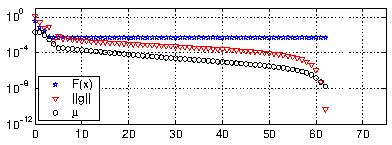
\includegraphics[width=0.72\linewidth]{assets/figures/fig-3-2a.pdf}
\begingroup
\setcounter{figure}{1}
\renewcommand{\thefigure}{3.2a}
\renewcommand{\theHfigure}{3.2a}
\caption{L-M 法用于例~1.1 中的拟合问题。}\label{fig:3.2a}\label{fig:3.2}
\endgroup
\end{figure}

为作比较，图~\ref{fig:3.2b} 给出了采用更新策略~\eqref{eq:2.20} 时的表现。从第 $5$ 步到第 $68$ 步，每次 $\mu$ 减小后都立即随之增大，梯度的范数也呈现出起伏不平的变化。这使收敛变慢，但最后阶段与图~\ref{fig:3.2a} 相同。

\begin{figure}[H]
\centering
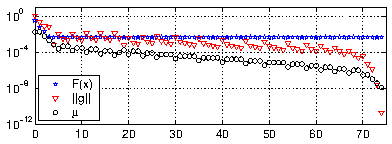
\includegraphics[width=0.72\linewidth]{assets/figures/fig-3-2b.pdf}
\begingroup
\setcounter{figure}{1}
\renewcommand{\thefigure}{3.2b}
\renewcommand{\theHfigure}{3.2b}
\caption{采用更新策略~\eqref{eq:2.20} 时的表现。}\label{fig:3.2b}
\endgroup
\end{figure}
\setcounter{figure}{2}
\end{example}

\begin{example}{3.8}
图~\ref{fig:3.3} 展示了将算法~3.16 用于例~3.2 和例~3.5 中 Powell 问题时的表现。初始点为 $\mathbf{x}_0=[3,1]^{\T}$，$\mu_0$ 由式~\eqref{eq:3.14} 中的 $\tau=1$ 给出，在停止准则~(3.15) 中取 $\varepsilon_1=\varepsilon_2=10^{-15}$、$k_{\max}=100$。

\sourcepage{29}
\begin{figure}[H]
\centering
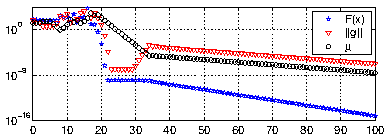
\includegraphics[width=0.72\linewidth]{assets/figures/fig-3-3.pdf}
\setcounter{figure}{2}
\caption{L-M 法用于 Powell 问题。}\label{fig:3.3}
\end{figure}

迭代在第 $22$ 步至第 $30$ 步之间似乎停滞了。这是 Jacobian 矩阵（几乎）奇异所造成的。此后似乎呈线性收敛。迭代由“保护条件”停止，停止点为 $\mathbf{x}=[-3.82\mathrm{e}{-08},-1.38\mathrm{e}{-03}]^{\T}$。这比在例~3.2 中得到的结果更接近 $\mathbf{x}^*=\mathbf{0}$，但我们希望还能做得更好，参见例~3.10 和例~3.17。
\end{example}

\section{Powell 狗腿法}\label{sec:dogleg}
与 Levenberg--Marquardt 法一样，这种方法也采用 Gauss--Newton 方向与最速下降方向的组合。不过，这里的控制是显式地通过信赖域的半径进行的，参见第~2.4 节。这一算法之所以与 Powell 的名字相联系，是因为他提出了求取式~\eqref{eq:2.23} 所定义的 $\mathbf{h}_{\mathrm{tr}}$ 的近似的方法。

给定 $\mathbf{f}:\R^n\to\R^m$。在当前迭代点 $\mathbf{x}$ 处，Gauss--Newton 步 $\mathbf{h}_{\mathrm{gn}}$ 是线性系统
\begin{equation}
  \mathbf{J}(\mathbf{x})\mathbf{h}\simeq-\mathbf{f}(\mathbf{x})
  \tag{3.17}\label{eq:3.17}
\end{equation}
的最小二乘解。它可以通过求解正规方程
\begin{equation}
  \bigl(\mathbf{J}(\mathbf{x})^{\T}\mathbf{J}(\mathbf{x})\bigr)\mathbf{h}_{\mathrm{gn}}=-\mathbf{J}(\mathbf{x})^{\T}\mathbf{f}(\mathbf{x})
  \tag{3.18a}\label{eq:3.18a}
\end{equation}
来计算。

最速下降方向由下式给出：
\begin{equation}
  \mathbf{h}_{\mathrm{sd}}=-\mathbf{g}=-\mathbf{J}(\mathbf{x})^{\T}\mathbf{f}(\mathbf{x}).
  \tag{3.18b}\label{eq:3.18b}
\end{equation}
这是一个方向，而非一个步。为确定应沿此方向走多远，我们考察线性模型
\sourcepage{30}
\[
\begin{aligned}
  &\mathbf{f}(\mathbf{x}+\alpha \mathbf{h}_{\mathrm{sd}})\simeq \mathbf{f}(\mathbf{x})+\alpha \mathbf{J}(\mathbf{x})\mathbf{h}_{\mathrm{sd}}\\
  &\Downarrow\\
  &F(\mathbf{x}+\alpha \mathbf{h}_{\mathrm{sd}})
     \simeq\tfrac12\norm{\mathbf{f}(\mathbf{x})+\alpha \mathbf{J}(\mathbf{x})\mathbf{h}_{\mathrm{sd}}}^2\\
  &\hphantom{F(\mathbf{x}+\alpha \mathbf{h}_{\mathrm{sd}})}
     =F(\mathbf{x})+\alpha \mathbf{h}_{\mathrm{sd}}^{\T}\mathbf{J}(\mathbf{x})^{\T}\mathbf{f}(\mathbf{x})
           +\tfrac12\alpha^2\norm{\mathbf{J}(\mathbf{x})\mathbf{h}_{\mathrm{sd}}}^2.
\end{aligned}
\]
这个关于 $\alpha$ 的函数在下列值处达到最小：
\begin{equation}
  \alpha=-\frac{\mathbf{h}_{\mathrm{sd}}^{\T}\mathbf{J}(\mathbf{x})^{\T}\mathbf{f}(\mathbf{x})}
                 {\norm{\mathbf{J}(\mathbf{x})\mathbf{h}_{\mathrm{sd}}}^2}
         =\frac{\norm{\mathbf{g}}^2}{\norm{\mathbf{J}(\mathbf{x})\mathbf{g}}^2}.
  \tag{3.19}\label{eq:3.19}
\end{equation}
现在，从当前点 $\mathbf{x}$ 出发的步有两个候选：$\mathbf{a}=\alpha \mathbf{h}_{\mathrm{sd}}$ 和 $\mathbf{b}=\mathbf{h}_{\mathrm{gn}}$。当信赖域半径为 $\Delta$ 时，Powell 提出采用以下策略选择步。策略中的最后一种情形如图~\ref{fig:3.4} 所示。
\begin{equation}
\begin{aligned}
 &\textbf{if}\quad \norm{\mathbf{h}_{\mathrm{gn}}}\leq\Delta\\
 &\qquad \mathbf{h}_{\mathrm{dl}}:=\mathbf{h}_{\mathrm{gn}}\\
 &\textbf{elseif}\quad \norm{\alpha \mathbf{h}_{\mathrm{sd}}}\geq\Delta\\
 &\qquad \mathbf{h}_{\mathrm{dl}}:=(\Delta/\norm{\mathbf{h}_{\mathrm{sd}}})\mathbf{h}_{\mathrm{sd}}\\
 &\textbf{else}\\
 &\qquad \mathbf{h}_{\mathrm{dl}}:=\alpha \mathbf{h}_{\mathrm{sd}}
                     +\beta(\mathbf{h}_{\mathrm{gn}}-\alpha \mathbf{h}_{\mathrm{sd}})\\
 &\qquad \text{其中选择 }\beta\text{ 使得 }\norm{\mathbf{h}_{\mathrm{dl}}}=\Delta.
\end{aligned}
\tag{3.20a}\label{eq:3.20a}
\end{equation}

\begin{figure}[H]
\centering
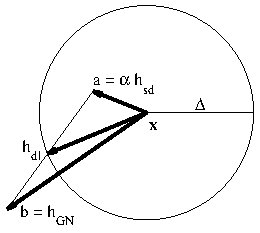
\includegraphics[width=0.44\linewidth]{assets/figures/fig-3-4.pdf}
\setcounter{figure}{3}
\caption{信赖域与狗腿步。\protect\footnotemark[4]}\label{fig:3.4}
\end{figure}
\footnotetext[4]{“狗腿”（Dog Leg）这一名称来自高尔夫球：在“狗腿洞”中，球道的形状就像从 $\mathbf{x}$（发球点）经过 $\mathbf{a}$ 的端点，再到 $\mathbf{h}_{\mathrm{dl}}$ 的端点（球洞）的折线。Powell 是一位热衷高尔夫球的人！}

\needspace{4\baselineskip}
\sourcepage{31}
令 $\mathbf{a}$、$\mathbf{b}$ 如上所定义，并令 $c=\mathbf{a}^{\T}(\mathbf{b}-\mathbf{a})$，则可写成
\[
 \psi(\beta)\equiv\norm{\mathbf{a}+\beta(\mathbf{b}-\mathbf{a})}^2-\Delta^2
 =\norm{\mathbf{b}-\mathbf{a}}^2\beta^2+2c\beta+\norm{\mathbf{a}}^2-\Delta^2.
\]
我们要找这个二次多项式的一个根。注意，$\beta\to-\infty$ 时 $\psi\to+\infty$；$\psi(0)=\norm{\mathbf{a}}^2-\Delta^2<0$；$\psi(1)=\norm{\mathbf{h}_{\mathrm{gn}}}^2-\Delta^2>0$。因此，$\psi$ 有一个负根和一个位于 $]0,1[$ 内的根。我们要找后者，最精确的计算方式为
\begin{equation}
\begin{aligned}
 &\textbf{if}\quad c\leq0\\
 &\quad\beta=
 \frac{-c+\sqrt{c^2+\norm{\mathbf{b}-\mathbf{a}}^2(\Delta^2-\norm{\mathbf{a}}^2)}}{\norm{\mathbf{b}-\mathbf{a}}^2}\\
 &\textbf{else}\\
 &\quad\beta=
 \frac{\Delta^2-\norm{\mathbf{a}}^2}
      {c+\sqrt{c^2+\norm{\mathbf{b}-\mathbf{a}}^2(\Delta^2-\norm{\mathbf{a}}^2)}}.
\end{aligned}
\tag{3.20b}\label{eq:3.20b}
\end{equation}
与 L-M 法一样，可以用增益比
\[
  \varrho=\bigl(F(\mathbf{x})-F(\mathbf{x}+\mathbf{h}_{\mathrm{dl}})\bigr)
            /\bigl(L(\mathbf{0})-L(\mathbf{h}_{\mathrm{dl}})\bigr)
\]
来监控迭代。这里，$L$ 仍然是线性模型
\[
  L(\mathbf{h})=\tfrac12\norm{\mathbf{f}(\mathbf{x})+\mathbf{J}(\mathbf{x})\mathbf{h}}^2.
\]
在 L-M 法中，我们用 $\varrho$ 控制阻尼参数的大小；这里则用它控制信赖域的半径 $\Delta$。较大的 $\varrho$ 值表示线性模型很好。这时可以增大 $\Delta$，从而走更长的步，且这些步更接近 Gauss--Newton 方向。若 $\varrho$ 很小（甚至为负），则减小 $\Delta$，这意味着步更短、方向更接近最速下降方向。下面概括这一算法。作如下说明。
\begin{enumerate}[label=$\arabic*^{\circ}$,leftmargin=2.2em]
\item 初始化。$\mathbf{x}_0$ 和 $\Delta_0$ 应由用户提供。
\item 采用停止准则~(3.15)，并补充 $\norm{\mathbf{f}(\mathbf{x})}_{\infty}\leq\varepsilon_3$，以体现当 $m=n$、即问题为非线性方程组时有 $\mathbf{f}(\mathbf{x}^*)=\mathbf{0}$。
\item 若 $m=n$，则将“$\simeq$”换成“$=$”，参见式~\eqref{eq:3.6}，并且不再绕道求解正规方程~\eqref{eq:3.18a}，参见例~3.9。
\end{enumerate}

\needspace{24\baselineskip}
\sourcepage{32}
\begin{algorithmbox}{3.21}{狗腿法}
\begin{tabbing}
\hspace{1.15em}\=\hspace{1.15em}\=\hspace{1.15em}\=\hspace{1.15em}\=\hspace{1.15em}\=\kill
\textbf{begin}\\
\> $k:=0;\quad \mathbf{x}:=\mathbf{x}_0;\quad\Delta:=\Delta_0;\quad \mathbf{g}:=\mathbf{J}(\mathbf{x})^{\T}\mathbf{f}(\mathbf{x})$\quad $\{1^{\circ}\}$\\
\> $\mathit{found}:=(\norm{\mathbf{f}(\mathbf{x})}_{\infty}\leq\varepsilon_3)$ \textbf{or}
   $(\norm{\mathbf{g}}_{\infty}\leq\varepsilon_1)$\quad $\{2^{\circ}\}$\\
\> \textbf{while} (\textbf{not} $\mathit{found}$) \textbf{and} $(k<k_{\max})$\\
\>\> $k:=k+1;$\quad 按式~\eqref{eq:3.19} 计算 $\alpha$\\
\>\> $\mathbf{h}_{\mathrm{sd}}:=-\alpha \mathbf{g};$\quad 求解 $\mathbf{J}(\mathbf{x})\mathbf{h}_{\mathrm{gn}}\simeq-\mathbf{f}(\mathbf{x})$\quad $\{3^{\circ}\}$\\
\>\> 按式~(3.20) 计算 $\mathbf{h}_{\mathrm{dl}}$\\
\>\> \textbf{if} $\norm{\mathbf{h}_{\mathrm{dl}}}\leq\varepsilon_2(\norm{\mathbf{x}}+\varepsilon_2)$\\
\>\>\> $\mathit{found}:=\mathbf{true}$\\
\>\> \textbf{else}\\
\>\>\> $\mathbf{x}_{\mathrm{new}}:=\mathbf{x}+\mathbf{h}_{\mathrm{dl}}$\\
\>\>\> $\varrho:=(F(\mathbf{x})-F(\mathbf{x}_{\mathrm{new}}))/(L(\mathbf{0})-L(\mathbf{h}_{\mathrm{dl}}))$\quad $\{4^{\circ}\}$\\
\>\>\> \textbf{if} $\varrho>0$\\
\>\>\>\> $\mathbf{x}:=\mathbf{x}_{\mathrm{new}};\quad \mathbf{g}:=\mathbf{J}(\mathbf{x})^{\T}\mathbf{f}(\mathbf{x})$\\
\>\>\>\> $\mathit{found}:=(\norm{\mathbf{f}(\mathbf{x})}_{\infty}\leq\varepsilon_3)$ \textbf{or}
   $(\norm{\mathbf{g}}_{\infty}\leq\varepsilon_1)$\\
\>\>\> \textbf{if} $\varrho>0.75$\qquad\qquad $\{5^{\circ}\}$\\
\>\>\>\> $\Delta:=\max\{\Delta,3*\norm{\mathbf{h}_{\mathrm{dl}}}\}$\\
\>\>\> \textbf{elseif} $\varrho<0.25$\\
\>\>\>\> $\Delta:=\Delta/2;\quad
 \mathit{found}:=(\Delta\leq\varepsilon_2(\norm{\mathbf{x}}+\varepsilon_2))$\quad $\{6^{\circ}\}$\\
\textbf{end}
\end{tabbing}
\end{algorithmbox}

\begin{enumerate}[label=$\arabic*^{\circ}$,leftmargin=2.2em,start=4]
\item 对应于式~\eqref{eq:3.20a} 中的三种情形，可以证明
\[
 L(\mathbf{0})-L(\mathbf{h}_{\mathrm{dl}})=
 \begin{cases}
  F(\mathbf{x}),&\text{若 }\mathbf{h}_{\mathrm{dl}}=\mathbf{h}_{\mathrm{gn}},\\[3pt]
  \dfrac{\Delta(2\norm{\alpha \mathbf{g}}-\Delta)}{2\alpha},
     &\text{若 }\mathbf{h}_{\mathrm{dl}}=-\dfrac{\Delta}{\norm{\mathbf{g}}}\mathbf{g},\\[7pt]
  \tfrac12\alpha(1-\beta)^2\norm{\mathbf{g}}^2+\beta(2-\beta)F(\mathbf{x}),
     &\text{其他情形。}
 \end{cases}
\]
\item 采用策略~\eqref{eq:2.19} 更新信赖域半径。
\item 附加的停止准则。若 $\Delta\leq\varepsilon_2(\norm{\mathbf{x}}+\varepsilon_2)$，则下一步一定满足式~\eqref{eq:3.15b}。
\end{enumerate}

\sourcepage{33}
\begin{example}{3.9}
例~3.6 简要讨论了步 $\mathbf{h}_{\mathrm{lm}}$ 的计算，并说明我们不妨通过正规方程形式~\eqref{eq:3.13} 来计算它。只要 $\mu$ 不是很小，矩阵的条件就较好，舍入误差不会产生过大的影响。

狗腿法旨在对非线性方程组也有良好的表现，即式~\eqref{eq:3.17} 是一个方形的线性方程组
\[
  \mathbf{J}(\mathbf{x})\mathbf{h}=-\mathbf{f}(\mathbf{x}),
\]
其解 $\mathbf{h}=\mathbf{h}_{\mathrm{nr}}$ 是 Newton--Raphson 步，参见例~3.2。Jacobian 矩阵 $\mathbf{J}$ 可能是病态的（甚至奇异），在这种情形下，舍入误差往往会主导所得的解。如果用式~\eqref{eq:3.18a} 来计算 $\mathbf{h}_{\mathrm{gn}}$，这个问题会更加严重。

\texttt{immoptibox} 中的 \texttt{dogleg} 实现在计算式~\eqref{eq:3.17} 的解时考虑了这些问题。如果 $\mathbf{J}(\mathbf{x})$ 的列没有显著的线性无关性，则最小二乘解 $\mathbf{h}$ 不唯一，这时把范数最小的 $\mathbf{h}$ 作为 $\mathbf{h}_{\mathrm{gn}}$。附录~B 给出了这种计算的一些细节。
\end{example}

\begin{example}{3.10}
图~\ref{fig:3.5} 展示了将狗腿法用于例~3.2 和例~3.8 中的 Powell 问题时的表现，其中初始点 $\mathbf{x}_0=[3,1]^{\T}$，$\Delta_0=1$，停止准则的参数为 $\varepsilon_1=\varepsilon_2=10^{-15}$、$\varepsilon_3=10^{-20}$、$k_{\max}=100$。

\begin{figure}[H]
\centering
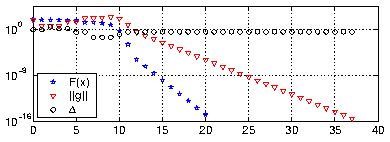
\includegraphics[width=0.72\linewidth]{assets/figures/fig-3-5.pdf}
\setcounter{figure}{4}
\caption{狗腿法用于 Powell 问题。}\label{fig:3.5}
\end{figure}

迭代在 $37$ 步后因梯度很小而停止，返回 $\mathbf{x}=[-2.41\cdot10^{-35},1.26\cdot10^{-9}]^{\T}$，这是 $\mathbf{x}^*=\mathbf{0}$ 的一个相当好的近似。与图~\ref{fig:3.3} 一样，可以看到最终是线性收敛（由 $\mathbf{J}(\mathbf{x}^*)$ 的奇异性引起），但明显快于 Marquardt 法。
\end{example}

% 原书印刷页 34--40；第 40 页的 3.5 节开头由下一文件承接。
\sourcepage{34}
\begin{example}{3.11}
我们将算法~3.21 用于例~1.1、3.4 和~3.7 中的数据拟合问题。与例~3.7 一样，取初始点
$\mathbf{x}_0=[-1,-2,1,-1]^{\T}$，并取 $\Delta_0=1$；停止准则的参数为
$\varepsilon_1=\varepsilon_2=\varepsilon_3=10^{-8}$、$k_{\max}=200$。
算法经过 30 次迭代后停止，得到 $\mathbf{x}\simeq[-4,-5,4,-4]^{\T}$。
其表现如下图所示。与图~3.3 一样，可以看到最终阶段的收敛速度非常快。

\begin{figure}[H]
  \centering
  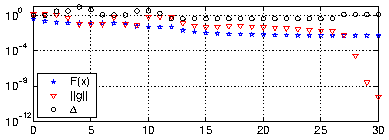
\includegraphics[width=0.68\linewidth]{assets/figures/fig-3-6.pdf}
  \setcounter{figure}{5}
  \caption{Dog Leg 法用于例~1.1 中的拟合问题。}
  \label{fig:3.6}
\end{figure}
\end{example}

上面两个例子似乎表明，Dog Leg 法远优于 Levenberg--Marquardt 法。
当最小二乘问题来自非线性方程组时，确实如此。目前，Dog Leg 法被认为是求解非线性方程组的最佳方法。

对于一般的最小二乘问题，Dog Leg 法与 L--M 法有同样的缺点：如果 $F(\mathbf{x}^*)\ne0$，
则预计最终阶段只能达到线性收敛，而且收敛缓慢。
对于给定的问题和给定的初始猜测 $\mathbf{x}_0$，无法预先判断这两种方法中哪一种更快。

\section{混合法：L--M 与拟 Newton 法}

1988 年，Madsen 提出了一种混合法，将 L--M 法与拟\setcounter{footnote}{4}\footnote{源自拉丁语：\textit{quasi} 意为“几乎”。拟 Newton 法的一般介绍见 Frandsen 等（2004）第~5~章。}
Newton 法结合起来。L--M 法在 $F(\mathbf{x}^*)=0$ 时二次收敛，否则线性收敛；
拟 Newton 法则即使在
\sourcepage{35}
$F(\mathbf{x}^*)\ne0$ 时也能超线性收敛。
迭代首先进行一系列 L--M 步。如果迭代的表现说明 $F(\mathbf{x}^*)$ 显著不为零，
就切换到拟 Newton 法，以获得更好的表现。
也可能出现迹象，说明切回 L--M 法更好，因此算法还设有相应的切换机制。

如果条件
\begin{equation}
  \norm{\mathbf{F}'(\mathbf{x})}_{\infty}<0.02\cdot F(\mathbf{x})
  \tag{3.22}\label{eq:3.22}
\end{equation}
在连续三个成功的迭代步中都成立，就切换到拟 Newton 法。
我们将这解释为一个迹象：迭代正在接近某个 $\mathbf{x}^*$，且该点满足
$\mathbf{F}'(\mathbf{x}^*)=\mathbf{0}$，而 $F(\mathbf{x}^*)$ 显著不为零。
如讨论式~\eqref{eq:3.12} 时所述，这可能导致缓慢的线性收敛。

拟 Newton 法的基础是，在当前迭代点 $\mathbf{x}$ 处有一个 Hessian 矩阵
$\mathbf{F}''(\mathbf{x})$ 的近似矩阵 $\mathbf{B}$；步向量 $\mathbf{h}_{\mathrm{qn}}$ 通过求解下式得到：
\begin{equation}
  \mathbf{B}\mathbf{h}_{\mathrm{qn}}=-\mathbf{F}'(\mathbf{x}).
  \tag{3.23}\label{eq:3.23}
\end{equation}
这是 Newton 方程~\eqref{eq:2.9a} 的近似形式。

近似矩阵 $\mathbf{B}$ 按照 BFGS 策略更新，参见 Frandsen 等（2004）第~5.10~节：
近似矩阵序列中的每一个 $\mathbf{B}$ 都是对称的（与任意 $\mathbf{F}''(\mathbf{x})$ 一样）且正定。
这保证了 $\mathbf{h}_{\mathrm{qn}}$ 是“下坡”方向，参见式~\eqref{eq:2.10}。
我们以对称正定矩阵 $\mathbf{B}_0=\mathbf{I}$ 为初始矩阵；BFGS 更新就是在当前 $\mathbf{B}$ 上加上一个秩二矩阵。
Madsen（1988）采用了 Al-Baali 和 Fletcher（1985）倡导的如下版本：
\begin{equation}
\begin{aligned}
  &\mathbf{h}:=\mathbf{x}_{\mathrm{new}}-\mathbf{x};\qquad
   \mathbf{y}:=\mathbf{J}_{\mathrm{new}}^{\T}\mathbf{J}_{\mathrm{new}}\mathbf{h}
        +(\mathbf{J}_{\mathrm{new}}-\mathbf{J})^{\T}\mathbf{f}(\mathbf{x}_{\mathrm{new}}),\\
  &\textbf{if }\mathbf{h}^{\T}\mathbf{y}>0\\
  &\qquad \mathbf{v}:=\mathbf{B}\mathbf{h};\qquad
    \mathbf{B}:=\mathbf{B}+\left(\frac{1}{\mathbf{h}^{\T}\mathbf{y}}\mathbf{y}\right)\mathbf{y}^{\T}
        -\left(\frac{1}{\mathbf{h}^{\T}\mathbf{v}}\mathbf{v}\right)\mathbf{v}^{\T}.
\end{aligned}
\tag{3.24}\label{eq:3.24}
\end{equation}
这里 $\mathbf{J}=\mathbf{J}(\mathbf{x})$，$\mathbf{J}_{\mathrm{new}}=\mathbf{J}(\mathbf{x}_{\mathrm{new}})$。
如前所述，当前的 $\mathbf{B}$ 是正定的，而且仅当 $\mathbf{h}^{\T}\mathbf{y}>0$ 时才改变它。
在这种情况下，可以证明新的 $\mathbf{B}$ 也正定。

\sourcepage{36}
拟 Newton 法在迭代的全局阶段并不稳健；不能保证它使目标函数下降。
在解 $\mathbf{x}^*$ 处有 $\mathbf{F}'(\mathbf{x}^*)=\mathbf{0}$，而 $\norm{\mathbf{F}'(\mathbf{x})}$ 的值迅速减小，
则表明最终阶段收敛良好。如果这些范数值减小得不够快，就切回 L--M 法。

算法概述如下。它调用辅助函数 \textit{LMstep} 和 \textit{QNstep}，分别实现这两种方法。

\begin{algorithmbox}{3.25}{混合法}
\label{alg:3.25}
\small
\begin{tabbing}
\qquad\=\qquad\=\qquad\=\qquad\=\qquad\=\kill
\textbf{begin}\\
\> $k:=0;\quad\mathbf{x}:=\mathbf{x}_0;\quad\mu:=\mu_0;\quad \mathbf{B}:=\mathbf{I}$
   \` $\{1^{\circ}\}$\\
\> $\mathit{found}:=(\norm{\mathbf{F}'(\mathbf{x})}_{\infty}\le\varepsilon_1);\quad
       \mathit{method}:=\text{L--M}$\\
\> \textbf{while} $(\textbf{not }\mathit{found})$ \textbf{and} $(k<k_{\max})$\\
\>\> $k:=k+1$\\
\>\> \textbf{case} $\mathit{method}$ \textbf{of}\\
\>\>\> L--M：\\
\>\>\>\> $[\mathbf{x}_{\mathrm{new}},\mathit{found},\mathit{better},\mathit{method},\ldots]
              :=\operatorname{LMstep}(\mathbf{x},\ldots)$
              \` $\{2^{\circ}\}$\\
\>\>\> Q--N：\\
\>\>\>\> $[\mathbf{x}_{\mathrm{new}},\mathit{found},\mathit{better},\mathit{method},\ldots]
              :=\operatorname{QNstep}(\mathbf{x},\mathbf{B},\ldots)$
              \` $\{2^{\circ}\}$\\
\>\> 按式~\eqref{eq:3.24} 更新 $\mathbf{B}$ \` $\{3^{\circ}\}$\\
\>\> \textbf{if} $\mathit{better}$\\
\>\>\> $\mathbf{x}:=\mathbf{x}_{\mathrm{new}}$\\
\textbf{end}
\end{tabbing}
\end{algorithmbox}

说明如下：
\begin{enumerate}[label=\(\arabic*^{\circ}\),leftmargin=2.8em]
  \item 初始化。$\mu_0$ 可由式~\eqref{eq:3.14} 确定。停止准则由式~\hyperref[eq:3.15a]{(3.15)} 给出。
  \item 省略号表示还传递 $\mathbf{f}$、$\mathbf{J}$ 等的当前值，从而不必对同一个 $\mathbf{x}$ 重复计算它们。
  \item 注意，L--M 步和拟 Newton 步都会为 Hessian 矩阵的近似提供信息。
\end{enumerate}
下面给出这两个辅助函数。

\needspace{24\baselineskip}
\sourcepage{37}
\begin{statement}{函数 3.26\quad Levenberg--Marquardt 步}
\label{fn:3.26}
\small
\[
  [\mathbf{x}_{\mathrm{new}},\mathit{found},\mathit{better},\mathit{method},\ldots]
       :=\operatorname{LMstep}(\mathbf{x},\ldots)
\]
\begin{tabbing}
\quad\=\quad\=\quad\=\quad\=\quad\=\quad\=\kill
\textbf{begin}\\
\> $\mathbf{x}_{\mathrm{new}}:=\mathbf{x};\quad\mathit{method}:=\text{L--M}$\\
\> 求解 $(\mathbf{J}(\mathbf{x})^{\T}\mathbf{J}(\mathbf{x})+\mu \mathbf{I})\mathbf{h}_{\mathrm{lm}}=-\mathbf{F}'(\mathbf{x})$\\
\> \textbf{if} $\norm{\mathbf{h}_{\mathrm{lm}}}\le\varepsilon_2(\norm{\mathbf{x}}+\varepsilon_2)$\\
\>\> $\mathit{found}:=\textbf{true}$\\
\> \textbf{else}\\
\>\> $\mathbf{x}_{\mathrm{new}}:=\mathbf{x}+\mathbf{h}_{\mathrm{lm}}$\\
\>\> $\varrho:=(F(\mathbf{x})-F(\mathbf{x}_{\mathrm{new}}))/(L(\mathbf{0})-L(\mathbf{h}_{\mathrm{lm}}))$
       \` $\{4^{\circ}\}$\\
\>\> \textbf{if} $\varrho>0$\\
\>\>\> $\mathit{better}:=\textbf{true};\quad
           \mathit{found}:=(\norm{\mathbf{F}'(\mathbf{x}_{\mathrm{new}})}_{\infty}\le\varepsilon_1)$\\
\>\>\> \textbf{if} $\norm{\mathbf{F}'(\mathbf{x}_{\mathrm{new}})}_{\infty}<0.02\cdot F(\mathbf{x}_{\mathrm{new}})$
         \` $\{5^{\circ}\}$\\
\>\>\>\> $\mathit{count}:=\mathit{count}+1$\\
\>\>\>\> \textbf{if} $\mathit{count}=3$ \` $\{6^{\circ}\}$\\
\>\>\>\>\> $\mathit{method}:=\text{Q--N}$\\
\>\>\> \textbf{else}\\
\>\>\>\> $\mathit{count}:=0$\\
\>\> \textbf{else}\\
\>\>\> $\mathit{count}:=0;\quad\mathit{better}:=\textbf{false}$\\
\textbf{end}
\end{tabbing}
\end{statement}

关于函数 \textit{LMstep} 和 \textit{QNstep}，还有以下说明：
\begin{enumerate}[label=\(\arabic*^{\circ}\),start=4,leftmargin=2.8em]
  \item 与算法~3.16 一样，增益比 $\varrho$ 还用于更新 $\mu$。
  \item 这是可能需要切换方法的迹象。参数 $\mathit{count}$ 在算法~3.25 开始时初始化为零。
  \item 式~\eqref{eq:3.22} 在连续三个迭代步中都成立，且这三步都有 $\varrho>0$，即每一步都改变了 $\mathbf{x}$。
\end{enumerate}

\needspace{24\baselineskip}
\sourcepage{38}
\begin{statement}{函数 3.27\quad 拟 Newton 步}
\label{fn:3.27}
\small
\[
  [\mathbf{x}_{\mathrm{new}},\mathit{found},\mathit{better},\mathit{method},\ldots]
       :=\operatorname{QNstep}(\mathbf{x},\mathbf{B},\ldots)
\]
\begin{tabbing}
\quad\=\quad\=\quad\=\quad\=\quad\=\kill
\textbf{begin}\\
\> $\mathbf{x}_{\mathrm{new}}:=\mathbf{x};\quad\mathit{method}:=\text{Q--N};\quad
       \mathit{better}:=\textbf{false}$\\
\> 求解 $\mathbf{B}\mathbf{h}_{\mathrm{qn}}=-\mathbf{F}'(\mathbf{x})$\\
\> \textbf{if} $\norm{\mathbf{h}_{\mathrm{qn}}}\le\varepsilon_2(\norm{\mathbf{x}}+\varepsilon_2)$\\
\>\> $\mathit{found}:=\textbf{true}$\\
\> \textbf{else}\\
\>\> \textbf{if} $\norm{\mathbf{h}_{\mathrm{qn}}}>\Delta$ \` $\{7^{\circ}\}$\\
\>\>\> $\mathbf{h}_{\mathrm{qn}}:=(\Delta/\norm{\mathbf{h}_{\mathrm{qn}}})\mathbf{h}_{\mathrm{qn}}$\\
\>\> $\mathbf{x}_{\mathrm{new}}:=\mathbf{x}+\mathbf{h}_{\mathrm{qn}}$\\
\>\> \textbf{if} $\norm{\mathbf{F}'(\mathbf{x}_{\mathrm{new}})}_{\infty}\le\varepsilon_1$
       \` $\{8^{\circ}\}$\\
\>\>\> $\mathit{found}:=\textbf{true}$\\
\>\> \textbf{else} \` $\{9^{\circ}\}$\\*
\>\>\> $\mathit{better}:=(F(\mathbf{x}_{\mathrm{new}})<F(\mathbf{x}))$ \textbf{or}\\*
\>\>\>\> $(F(\mathbf{x}_{\mathrm{new}})\le(1+\delta)F(\mathbf{x})$\\*
\>\>\>\> \textbf{and} $\norm{\mathbf{F}'(\mathbf{x}_{\mathrm{new}})}_{\infty}<\norm{\mathbf{F}'(\mathbf{x})}_{\infty})$\\
\>\>\> \textbf{if} $\norm{\mathbf{F}'(\mathbf{x}_{\mathrm{new}})}_{\infty}\ge\norm{\mathbf{F}'(\mathbf{x})}_{\infty}$
         \` $\{10^{\circ}\}$\\
\>\>\>\> $\mathit{method}:=\text{L--M}$\\
\textbf{end}
\end{tabbing}
\end{statement}

\begin{enumerate}[label=\(\arabic*^{\circ}\),start=7,leftmargin=2.8em]
  \item 我们将拟 Newton 法与信赖域方法结合起来，并对约束起作用的情形作简单处理，
        参见第~\pageref{src:15}~页及下一页。从 L--M 法切换过来时，$\Delta$ 初始化为
        \[
          \max\left\{1.5\varepsilon_2(\norm{\mathbf{x}}+\varepsilon_2),\;
                      \frac{1}{5}\norm{\mathbf{h}_{\mathrm{lm}}}\right\}.
        \]
  \item 未在伪代码中列出：用式~\eqref{eq:2.19} 更新 $\Delta$。
  \item 在算法的这一部分，我们着重于使 $\mathbf{F}'$ 更接近于零，因此允许 $F$ 的值略微增大。
        例如，可取 $\delta=\sqrt{\varepsilon_M}$，其中 $\varepsilon_M$ 是计算机的单位舍入误差。
  \item 梯度减小得不够快。
\end{enumerate}

\sourcepage{39}
\begin{example}{3.12}
注意，更新公式~\eqref{eq:3.24} 中 $\mathbf{y}$ 的计算涉及乘积
$\mathbf{J}(\mathbf{x})^{\T}\mathbf{f}(\mathbf{x}_{\mathrm{new}})$。
这意味着我们必须保存前一次的 Jacobian 矩阵。也可以在更新公式中改用
\[
  \mathbf{y}=\mathbf{F}'(\mathbf{x}_{\mathrm{new}})-\mathbf{F}'(\mathbf{x})=\mathbf{g}_{\mathrm{new}}-\mathbf{g},
\]
不过 Madsen（1988）发现，式~\eqref{eq:3.24} 的表现更好。

Madsen（1988）的拟 Newton 步没有包含信赖域处理；但在开发 immoptibox 函数
\texttt{nlshybrid} 的过程中，发现这一想法能够改善算法表现。
它减少了无效尝试 Q--N 步的次数；所谓无效尝试，是指第~$10^{\circ}$~条中的条件立即使算法返回 L--M 法。
\end{example}

\begin{example}{3.13}
对于例~3.7 和~3.8 讨论的问题，这种混合法不会优于算法~3.16。
在后一种情形中（见图~3.3），$F(\mathbf{x})\to0$，说明~$5^{\circ}$~中的切换条件永远不会满足。
在前一种情形中，$F(\mathbf{x}^*)$ 显著不为零，但是，正如例~3.7 所讨论的，
简单的 L--M 法已经具有所需的最终超线性收敛性。

为展示算法~3.25 的效率，我们考虑修正的 Rosenbrock 问题，参见 Frandsen 等（1999）例~5.5。
该问题由 $\mathbf{f}:\R^2\to\R^3$ 给出，其中
\[
  \mathbf{f}(\mathbf{x})=
  \begin{bmatrix}
    10(x_2-x_1^2)\\
    1-x_1\\
    \lambda
  \end{bmatrix},
\]
参数 $\lambda$ 可以选择。
$F(\mathbf{x})=\tfrac12\mathbf{f}(\mathbf{x})^{\T}\mathbf{f}(\mathbf{x})$ 的极小点为
$\mathbf{x}^*=[1,1]^{\T}$，且 $F(\mathbf{x}^*)=\tfrac12\lambda^2$。

下面给出若干 $\lambda$ 值下算法~3.16 和~3.25 的结果。
在所有情形中，都取 $\mathbf{x}_0=[-1.2,1]^{\T}$；初始阻尼参数 $\mu_0$ 由
式~\eqref{eq:3.14} 定义，其中 $\tau=10^{-3}$；停止准则~\hyperref[eq:3.15a]{(3.15)} 中取
$(\varepsilon_1,\varepsilon_2,k_{\max})=(10^{-10},10^{-14},200)$。

在前两种情形中，$\lambda$ 太小，不会真正影响迭代；但当 $\lambda$ 较大时，
可以看到混合法远优于简单的 Levenberg--Marquardt 算法，尤其是在所获得的精度方面。

图~\ref{fig:3.7} 展示了 $\lambda=10^4$ 时这两种算法的表现。

\sourcepage{40}
\begin{center}
\small
\begin{tabular}{|c|rr|rr|}
  \cline{2-5}
  \multicolumn{1}{c|}{} & \multicolumn{2}{c|}{算法 3.16} & \multicolumn{2}{c|}{算法 3.25}\\
  \hline
  $\lambda$ & 迭代步数 & $\norm{\mathbf{x}-\mathbf{x}^*}$ & 迭代步数 & $\norm{\mathbf{x}-\mathbf{x}^*}$\\
  \hline
  $0$       & 17 & $2.78\times10^{-12}$ & 17 & $2.78\times10^{-12}$\\
  $10^{-5}$ & 17 & $2.78\times10^{-12}$ & 17 & $2.78\times10^{-12}$\\
  $1$       & 24 & $1.69\times10^{-9}$  & 19 & $2.23\times10^{-14}$\\
  $10^2$    & 23 & $5.87\times10^{-7}$  & 22 & $3.16\times10^{-12}$\\
  $10^4$    & 23 & $2.37\times10^{-4}$  & 22 & $3.16\times10^{-12}$\\
  \hline
\end{tabular}
\end{center}

\begin{figure}[H]
  \centering
  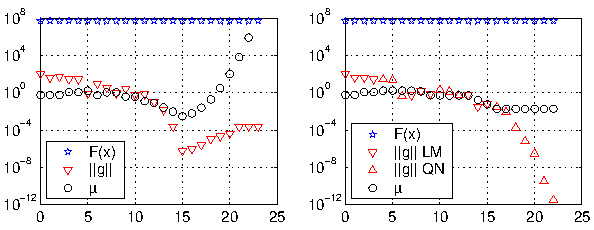
\includegraphics[width=0.96\linewidth]{assets/figures/fig-3-7.pdf}
  \setcounter{figure}{6}
  \caption{Levenberg--Marquardt 法（左）与混合法（右）。}
  \label{fig:3.7}
\end{figure}

使用 L--M 法时，第 15 步之后的所有步骤都未能改善目标函数；
$\mu$ 迅速增大，第 23 步满足停止准则~\eqref{eq:3.15b}，迭代因而终止。

使用混合法时，分别从第 5、11 和 17 步开始，多次尝试使用拟 Newton 法。
最后一次尝试成功，经过 22 步后，迭代由式~\eqref{eq:3.15a} 停止。
\end{example}

% 原书第 40 页末尾至第 49 页；第 40 页的 sourcepage 标记由前一分稿提供。
\section{L--M 法的割线版本}\label{sec:secant-lm}
本书讨论的方法都假定向量函数 $\mathbf f$ 可微，也就是说，雅可比矩阵
\[
  \mathbf J(\mathbf x)=\left[\frac{\partial f_i}{\partial x_j}\right]
\]
存在。在许多实际优化问题中，我们无法给出 $\mathbf J$ 中各元素的公式，例如 $\mathbf f$ 是由一个“黑箱”给出的。L--M 法的割线版本就是为这类问题设计的。

\sourcepage{41}
最简单的补救办法，是用通过\emph{数值微分}得到的矩阵 $\mathbf B$ 代替 $\mathbf J(\mathbf x)$：第 $(i,j)$ 个元素用有限差分近似式
\begin{equation}
  \frac{\partial f_i}{\partial x_j}(\mathbf x)
  \simeq \frac{f_i(\mathbf x+\delta\mathbf e_j)-f_i(\mathbf x)}{\delta}
  \equiv b_{ij},
  \tag{3.28}\label{eq:3.28}
\end{equation}
来近似。其中，$\mathbf e_j$ 是第 $j$ 个坐标方向上的单位向量，$\delta$ 是一个适当小的实数。采用这种策略，每个迭代点 $\mathbf x$ 都需要计算 $n+1$ 次 $\mathbf f$；而由于 $\delta$ 很可能远小于距离 $\norm{\mathbf x-\mathbf x^*}$，所得到的关于 $\mathbf f$ 全局行为的信息，也不会比仅计算 $\mathbf f(\mathbf x)$ 多出多少。我们希望有更高的效率。

\begin{example}{3.14}
令 $m=n=1$，考虑一个非线性方程
\[
  f:\R\mapsto\R.\qquad \text{求 }\widehat{x}\text{，使 }f(\widehat{x})=0.
\]
对于这个问题，可以将牛顿--拉夫森算法（3.6）写成
\begin{equation}
  \begin{aligned}
    &f(x+h)\simeq\ell(h)\equiv f(x)+f'(x)h,\\
    &\text{求解线性问题 }\ell(h)=0,\\
    &x_{\mathrm{new}}:=x+h.
  \end{aligned}
  \tag{3.29}\label{eq:3.29}
\end{equation}
如果无法实现 $f'(x)$，可以用
\[
  \bigl(f(x+\delta)-f(x)\bigr)/\delta
\]
来近似它，其中 $\delta$ 选取得适当小。更一般地，可以将式~\eqref{eq:3.29} 替换为
\begin{equation}
  \begin{aligned}
    &f(x+h)\simeq\lambda(h)\equiv f(x)+bh,
      \qquad\text{其中 }b\simeq f'(x),\\
    &\text{求解线性问题 }\lambda(h)=0,\\
    &x_{\mathrm{new}}:=x+h.
  \end{aligned}
  \tag{3.30a}\label{eq:3.30a}
\end{equation}
假定已经知道 $x_{\mathrm{prev}}$ 和 $f(x_{\mathrm{prev}})$。那么，可以通过要求
\begin{equation}
  f(x_{\mathrm{prev}})=\lambda(x_{\mathrm{prev}}-x)
  \tag{3.30b}\label{eq:3.30b}
\end{equation}
来确定因子 $b$，也就是 $f'(x)$ 的近似。这给出
$b=\bigl(f(x)-f(x_{\mathrm{prev}})\bigr)/(x-x_{\mathrm{prev}})$。
采用这个 $b$，便可看出（3.30）就是\emph{割线法}，例如可参见 Eldén 等（2004）第 70 页及后续内容。

\sourcepage{42}
与使用另一种有限差分近似的牛顿--拉夫森法相比，割线法的主要优点在于，每次迭代只需计算一次函数值，而不是两次。
\end{example}

现在，考虑 $\mathbf f:\R^n\mapsto\R^m$ 的线性模型（3.7a），
\[
  \mathbf f(\mathbf x+\mathbf h)\simeq\boldsymbol{\ell}(\mathbf h)
  \equiv\mathbf f(\mathbf x)+\mathbf J(\mathbf x)\mathbf h.
\]
我们将其替换为
\[
  \mathbf f(\mathbf x+\mathbf h)\simeq\boldsymbol{\lambda}(\mathbf h)
  \equiv\mathbf f(\mathbf x)+\mathbf B\mathbf h,
\]
其中 $\mathbf B$ 是当前对 $\mathbf J(\mathbf x)$ 的近似。在下一次迭代中，需要 $\mathbf B_{\mathrm{new}}$ 满足
\[
  \mathbf f(\mathbf x_{\mathrm{new}}+\mathbf h)
  \simeq\mathbf f(\mathbf x_{\mathrm{new}})+\mathbf B_{\mathrm{new}}\mathbf h.
\]
特别地，我们希望当 $\mathbf h=\mathbf x-\mathbf x_{\mathrm{new}}$ 时，这个模型的等式精确成立，即
\begin{equation}
  \mathbf f(\mathbf x)=\mathbf f(\mathbf x_{\mathrm{new}})
    +\mathbf B_{\mathrm{new}}(\mathbf x-\mathbf x_{\mathrm{new}}).
  \tag{3.31a}\label{eq:3.31a}
\end{equation}
这为 $\mathbf B_{\mathrm{new}}$ 中的 $m\cdot n$ 个未知元素给出了 $m$ 个方程，因此还需要更多条件。Broyden（1965）建议，在式~\eqref{eq:3.31a} 之外补充
\begin{equation}
  \mathbf B_{\mathrm{new}}\mathbf v=\mathbf B\mathbf v
  \qquad\text{对所有 }\mathbf v\perp(\mathbf x-\mathbf x_{\mathrm{new}}).
  \tag{3.31b}\label{eq:3.31b}
\end{equation}
容易验证，下面的更新满足条件（3.31a--b）。

\begin{statement}{定义 3.32\quad Broyden 秩一更新}\label{def:3.32}
\[
  \mathbf B_{\mathrm{new}}=\mathbf B+\mathbf u\mathbf h^{\T},
\]
其中
\[
  \mathbf h=\mathbf x_{\mathrm{new}}-\mathbf x,\qquad
  \mathbf u=\frac{1}{\mathbf h^{\T}\mathbf h}
    \bigl(\mathbf f(\mathbf x_{\mathrm{new}})-\mathbf f(\mathbf x)-\mathbf B\mathbf h\bigr).
\]
\end{statement}

注意，在 $n=1$ 时，条件~\eqref{eq:3.31a} 对应于割线条件~\eqref{eq:3.30b}。我们称这种方法为\emph{广义割线法}。采用这一修改后，算法 3.16 核心部分的简要形式为

\sourcepage{43}
\[
  \begin{aligned}
    &\text{求解 }(\mathbf B^{\T}\mathbf B+\mu\mathbf I)\mathbf h_{\mathrm{slm}}
       =-\mathbf B^{\T}\mathbf f(\mathbf x),\\
    &\mathbf x_{\mathrm{new}}:=\mathbf x+\mathbf h_{\mathrm{slm}},\\
    &\text{按（3.32）更新 }\mathbf B,\\
    &\text{按算法 3.16 更新 }\mu\text{ 和 }\mathbf x.
  \end{aligned}
\]
Powell 已经证明，如果向量序列 $\mathbf x_0,\mathbf x_1,\mathbf x_2,\ldots$ 收敛到 $\mathbf x^*$，而且步长向量序列 $\{\mathbf h_k\equiv\mathbf x_k-\mathbf x_{k-1}\}$ 满足如下条件：对于每个 $k\geq n$，$\{\mathbf h_{k-n+1},\ldots,\mathbf h_k\}$ 都线性无关，也就是说，它们张成整个 $\R^n$，那么，无论 $\mathbf B_0$ 如何选择，近似矩阵序列 $\{\mathbf B_k\}$ 都收敛到 $\mathbf J(\mathbf x^*)$。

然而，在实际计算中，前 $n$ 个步长向量往往不能张成整个 $\R^n$。因此存在这样一种风险：迭代若干步后，当前 $\mathbf B$ 对真实雅可比矩阵的近似很差，以至于 $-\mathbf B^{\T}\mathbf f(\mathbf x)$ 甚至不是一个下降方向。在这种情况下，$\mathbf x$ 将保持不变，而 $\mu$ 增大。近似矩阵 $\mathbf B$ 虽然也发生改变，但仍可能是一个很差的近似，从而导致 $\mu$ 进一步增大，如此继续下去。最终，$\mathbf h_{\mathrm{slm}}$ 变得很小，使得（3.15b）成立，于是过程停止，尽管此时 $\mathbf x$ 可能还远离 $\mathbf x^*$。

为克服这个问题，人们提出了许多策略，例如偶尔用有限差分重新计算 $\mathbf B$。在下面的算法 3.34 中，除了随迭代过程确定的更新外，我们还加入一组按坐标循环进行的更新：设 $\mathbf h$ 表示当前步长向量，$j$ 表示当前坐标编号。如果 $\mathbf h$ 与 $\mathbf e_j$ 的夹角 $\theta$ “很大”，就计算 $\mathbf J$ 第 $j$ 列的有限差分近似。具体地说，当
\begin{equation}
  \cos\theta=\frac{|\mathbf h^{\T}\mathbf e_j|}
    {\norm{\mathbf h}\cdot\norm{\mathbf e_j}}<\gamma
  \quad\Longleftrightarrow\quad |h_j|<\gamma\norm{\mathbf h}
  \tag{3.33}\label{eq:3.33}
\end{equation}
时，就进行这个计算。

实验表明，取 $\gamma=0.8$ 这一相当保守的数值，能够获得良好的表现。作此选择时，可以预期每次迭代需要计算向量函数 $\mathbf f$（几乎）两次。

现在可以给出算法了。阻尼参数 $\mu$ 的控制与算法 3.16 相同，为使表达清楚，下面不再列出。

\needspace{24\baselineskip}
\sourcepage{44}
\begin{algorithmbox}{3.34}{L--M 法的割线版本}\label{alg:3.34}
\small
\begin{tabbing}
  \qquad\=\qquad\=\qquad\=\qquad\=\kill
  \textbf{begin}\\
  \> $k:=0;\quad\mathbf x:=\mathbf x_0;\quad\mathbf B:=\mathbf B_0;\quad j:=0$
       \qquad $\{1^\circ\}$\\
  \> $\mathbf g:=\mathbf B^{\T}\mathbf f(\mathbf x);\quad
       \mathit{found}=(\norm{\mathbf g}_{\infty}\leq\varepsilon_1)$\\
  \> \textbf{while} $\bigl(\textbf{not }\mathit{found}\bigr)$
       \textbf{and} $(k<k_{\max})$\\
  \>\> $k:=k+1;$\quad 求解 $(\mathbf B^{\T}\mathbf B+\mu\mathbf I)\mathbf h=-\mathbf g$\\
  \>\> \textbf{if} $\norm{\mathbf h}\leq\varepsilon_2(\norm{\mathbf x}+\varepsilon_2)$\\
  \>\>\> $\mathit{found}:=\mathit{true}$\\
  \>\> \textbf{else}\\
  \>\>\> $j:=\operatorname{mod}(j,n)+1;$\quad
       \textbf{if} $|h_j|<0.8\norm{\mathbf h}$\quad $\{2^\circ\}$\\
  \>\>\>\> 按（3.32）更新 $\mathbf B$，取 $\mathbf x_{\mathrm{new}}=\mathbf x+\eta\mathbf e_j$
       \quad $\{3^\circ\}$\\
  \>\>\> $\mathbf x_{\mathrm{new}}:=\mathbf x+\mathbf h;$\quad 按（3.32）更新 $\mathbf B$\\
  \>\>\> \textbf{if} $F(\mathbf x_{\mathrm{new}})<F(\mathbf x)$\\
  \>\>\>\> $\mathbf x:=\mathbf x_{\mathrm{new}}$\\
  \>\> $\mathbf g:=\mathbf B^{\T}\mathbf f(\mathbf x);\quad
       \mathit{found}:=(\norm{\mathbf g}_{\infty}\leq\varepsilon_1)$
       \quad $\{4^\circ\}$\\
  \textbf{end}
\end{tabbing}
\end{algorithmbox}

有以下几点说明：
\begin{enumerate}[label=$\arabic*^\circ$,leftmargin=2.4em]
  \item 初始化。$\mathbf x_0$ 为输入值；$\mathbf B_0$ 可以作为输入给出，也可以由式~\eqref{eq:3.28} 计算。停止准则（3.15）中的参数，以及式~\eqref{eq:3.28} 所用的步长 $\delta$，同样都是输入值。
  \item 参见式~\eqref{eq:3.33}。$\operatorname{mod}(j,n)$ 是 $j$ 除以 $n$ 所得的余数。
  \item 步长 $\eta$ 由下式给出：
    \[
      \textbf{if }x_j=0\ \textbf{then }\eta:=\delta^2
      \ \textbf{else }\eta:=\delta|x_j|.
    \]
  \item 迭代点 $\mathbf x$ 只有在满足下降条件（2.1）时才更新，而近似矩阵 $\mathbf B$ 每一步都更新。因此，即使 $\mathbf f(\mathbf x)$ 保持不变，近似梯度 $\mathbf g$ 也可能发生改变。
\end{enumerate}

\begin{example}{3.15}
我们将算法 3.34 用于例 3.13 中 $\lambda=0$ 的修改 Rosenbrock 问题。如果使用与该例相同的初始点和停止准则，并在差分近似
\sourcepage{45}
式~\eqref{eq:3.28} 中取 $\delta=10^{-7}$，那么经 29 次迭代后得到解，总共计算了 53 次 $\mathbf f(\mathbf x)$。相比之下，“真正的”L--M 算法只需要 17 步，也就是总共计算 18 次 $\mathbf f(\mathbf x)$ 和 $\mathbf J(\mathbf x)$。

我们还将割线算法用于例 1.1、3.7 和 3.11 中的数据拟合问题。取 $\delta=10^{-7}$，并使用与例 3.7 相同的初始点和停止准则，迭代经过 94 步后因满足（3.15a）而停止，总共计算了 192 次 $\mathbf f(\mathbf x)$。相比之下，算法 3.16 需要 62 次迭代。

这两个问题表明，算法 3.34 是稳健的；同时也说明了一条普遍的经验法则：如果能够获得梯度信息，使用它通常是划算的。
\end{example}

在许多应用中，$m$ 和 $n$ 都很大，但每个函数 $f_i(\mathbf x)$ 只依赖于 $\mathbf x$ 中的少数几个元素。此时，大多数 $\frac{\partial f_i}{\partial x_j}(\mathbf x)$ 都为零，我们称 $\mathbf J(\mathbf x)$ 为\emph{稀疏矩阵}。对于 Levenberg--Marquardt 方程（3.13）的求解，已有利用稀疏性的高效方法，例如可参见 Nielsen（1997）。然而，在更新公式（3.32）中，向量 $\mathbf h$ 和 $\mathbf u$ 的元素通常全部非零，因此 $\mathbf B_{\mathrm{new}}$ 将成为稠密矩阵。如何处理这种情况，超出了本书的范围；读者可参见 Gill 等（1984）和 Toint（1987）。

\section{Dog Leg 法的割线版本}\label{sec:secant-dogleg}
当然，采用雅可比矩阵割线近似的思想，也可以用于第 3.3 节的 Dog Leg 法。本节考虑 $m=n$ 这一特殊情形，也就是求解非线性方程组。Broyden（1965）不仅给出了定义 3.32 中用于更新近似雅可比矩阵的公式
\begin{equation}
  \begin{aligned}
    \mathbf B_{\mathrm{new}}&=\mathbf B+
      \left(\frac{1}{\mathbf h^{\T}\mathbf h}(\mathbf y-\mathbf B\mathbf h)\right)\mathbf h^{\T},\\
    &\text{其中 }\mathbf h=\mathbf x_{\mathrm{new}}-\mathbf x,\qquad
      \mathbf y=\mathbf f(\mathbf x_{\mathrm{new}})-\mathbf f(\mathbf x),
  \end{aligned}
  \tag{3.35a}\label{eq:3.35a}
\end{equation}
还给出了更新雅可比矩阵近似逆 $\mathbf D\simeq\mathbf J(\mathbf x)^{-1}$ 的公式。该公式为

\sourcepage{46}
\begin{equation}
  \mathbf D_{\mathrm{new}}=\mathbf D+
    \left(\frac{1}{\mathbf h^{\T}\mathbf D\mathbf y}(\mathbf h-\mathbf D\mathbf y)\right)
    (\mathbf h^{\T}\mathbf D),
  \tag{3.35b}\label{eq:3.35b}
\end{equation}
其中 $\mathbf h$ 和 $\mathbf y$ 的定义见式~\eqref{eq:3.35a}。

利用这些矩阵，可以将最速下降方向 $\mathbf h_{\mathrm{sd}}$ 和 Gauss--Newton 步 $\mathbf h_{\mathrm{gn}}$（3.18）近似为
\begin{equation}
  \mathbf h_{\mathrm{ssd}}=-\mathbf B^{\T}\mathbf f(\mathbf x),
  \qquad\text{以及}\qquad
  \mathbf h_{\mathrm{sgn}}=-\mathbf D\mathbf f(\mathbf x).
  \tag{3.36}\label{eq:3.36}
\end{equation}
在这里，Gauss--Newton 步与牛顿步相同，参见例 3.5。

只需稍作修改，算法 3.21 就可以使用这些近似。初始矩阵 $\mathbf B=\mathbf B_0$ 可以由差分近似式~\eqref{eq:3.28} 得到，而 $\mathbf D_0$ 则计算为 $\mathbf B_0^{-1}$。容易证明，此后当前的 $\mathbf B$ 和 $\mathbf D$ 满足 $\mathbf B\mathbf D=\mathbf I$。步长参数 $\alpha$ 由式（3.19）求得，其中将 $\mathbf J(\mathbf x)$ 替换为 $\mathbf B$。

与 L--M 法的割线版本相同，这个方法也需要额外的更新，以使 $\mathbf B$ 和 $\mathbf D$ 始终分别是当前雅可比矩阵及其逆的良好近似。我们发现，围绕式~\eqref{eq:3.33} 所讨论的策略，在这里也很有效。还应指出，式~\eqref{eq:3.35b} 中的分母可能为零或非常小。如果
\[
  \left|\mathbf h^{\T}\mathbf D\mathbf y\right.
    <\sqrt{\varepsilon_M}\,\norm{\mathbf h},
\]
就不再更新 $\mathbf D$，而是将其计算为 $\mathbf D=\mathbf B^{-1}$。

每次按式（3.35）更新的“代价”为 $10n^2$ 次浮点运算\footnote[6]{一次“浮点运算”（flop）是两个浮点数之间的一次简单算术运算。}；而利用式~\eqref{eq:3.36} 计算两个步长向量，再加上按式（3.19）计算 $\alpha$，需要 $6n^2$ 次浮点运算。因此，Dog Leg 法的无梯度版本每次迭代的代价约为 $16n^2$ 次浮点运算，再加上计算 $\mathbf f(\mathbf x_{\mathrm{new}})$ 的代价。相比之下，算法 3.21 每一步的代价约为 $\frac{2}{3}n^3+6n^2$ 次浮点运算，再加上计算 $\mathbf f(\mathbf x_{\mathrm{new}})$ 和 $\mathbf J(\mathbf x_{\mathrm{new}})$ 的代价。因此，当 $n$ 很大时，无梯度版本每一步的代价更低。然而，它所需的迭代次数往往多得多；如果能够获得雅可比矩阵，采用梯度的版本通常更快。

\sourcepage{47}
\begin{example}{3.16}
我们将算法 3.21 和无梯度 Dog Leg 法用于 Rosenbrock 函数 $\mathbf f:\R^2\mapsto\R^2$，其定义为
\[
  \mathbf f(\mathbf x)=
    \begin{bmatrix}10(x_2-x_1^2)\\1-x_1\end{bmatrix},
\]
参见例 3.13。该函数只有一个根，$\mathbf x^*=[\,1,1\,]^{\T}$。对于两种方法，我们都采用初始点 $\mathbf x_0=[\,-1.2,1\,]^{\T}$，在停止准则（3.15）中取 $\varepsilon_1=\varepsilon_2=10^{-12}$、$k_{\max}=100$，并在式~\eqref{eq:3.28} 中取 $\delta=10^{-7}$。算法 3.21 经 17 次迭代后在解处停止，也就是说，计算了 18 次 $\mathbf f$ 及其雅可比矩阵。割线版本同样在解处停止；它需要 28 次迭代，总共计算了 49 次 $\mathbf f$。
\end{example}

\section{最后说明}\label{sec:final-remarks}
我们已经讨论了多种求解非线性最小二乘问题的算法。任何好的程序库中都有这些算法，也可以通过 GAMS（Guide to Available Mathematical Software，可用数学软件指南）查找相应的实现，其网址为
\begin{center}
  \url{http://gams.nist.gov}
\end{center}
本书中的例子使用 MATLAB 进行计算。相关程序包含在工具箱 immoptibox 中，可从下列网址获得：
\begin{center}
  \url{http://www.imm.dtu.dk/~hbn/immoptibox}
\end{center}
最后还应指出，有时重新表述问题，可以使问题更容易求解。下面用几个例子说明这一点，其中的思想也可能适用于读者自己的问题。

\begin{example}{3.17}
在例 3.2、3.8 和 3.10 的 Powell 问题中，变量 $x_2$ 只以 $x_2^2$ 的形式出现。可以引入新变量 $\mathbf z=[\,x_1,x_2^2\,]^{\T}$，问题便成为：求 $\mathbf z^*\in\R^2$，使 $\mathbf f(\mathbf z^*)=\mathbf0$，其中
\[
  \mathbf f(\mathbf z)=
    \begin{bmatrix}z_1\\\dfrac{10z_1}{z_1+0.1}+2z_2\end{bmatrix},
  \qquad\text{且}\qquad
  \mathbf J(\mathbf z)=
    \begin{bmatrix}1&0\\(z_1+0.1)^{-2}&2\end{bmatrix}.
\]
这个雅可比矩阵对所有 $\mathbf z$ 都非奇异。使用 L--M 算法 3.16，取初始点 $\mathbf z_0=[\,3,1\,]^{\T}$、$\tau=10^{-16}$，并在停止准则
\sourcepage{48}
（3.15）中取 $\varepsilon_1=\varepsilon_2=10^{-15}$，经 3 步后停止，得到
\mbox{$\mathbf z\simeq[\,\text{\ttfamily -1.40e-25},\text{\ttfamily 9.77e-25}\,]^{\T}$}。
这是对 $\mathbf z^*=\mathbf0$ 的良好近似。
\end{example}

\begin{example}{3.18}
例 1.1、3.7 和 3.11 中的数据拟合问题可以重新表述为仅含两个参数 $x_1$ 和 $x_2$ 的问题：将模型写成
\[
  M(\mathbf x,t)=c_1\mathrm e^{x_1t}+c_2\mathrm e^{x_2t},
\]
其中，对给定的 $\mathbf x$，向量 $\mathbf c=\mathbf c(\mathbf x)\in\R^2$ 是线性问题
\[
  \mathbf E\mathbf c\simeq\mathbf y
\]
的最小二乘解。这里，$\mathbf E=\mathbf E(\mathbf x)\in\R^{m\times2}$ 的各行由
$(\mathbf E)_{i,:}=[\,\mathrm e^{x_1t_i}\ \mathrm e^{x_2t_i}\,]$
给出。与例 1.1 一样，函数 $\mathbf f$ 的定义为 $f_i(\mathbf x)=y_i-M(\mathbf x,t_i)$，从而有
\[
  \mathbf f(\mathbf x)=\mathbf y-\mathbf E(\mathbf x)\mathbf c(\mathbf x).
\]
可以证明，其雅可比矩阵为
\[
  \mathbf J=-\mathbf E\mathbf G-\mathbf H[\mathbf c],
\]
其中，对于任意向量 $\mathbf u$，定义对角矩阵 $[\mathbf u]=\operatorname{diag}(\mathbf u)$，并且
\[
  \mathbf H=[\mathbf t]\mathbf E,\qquad
  \mathbf G=(\mathbf E^{\T}\mathbf E)^{-1}
    \bigl([\mathbf H^{\T}\mathbf f]-\mathbf H^{\T}\mathbf E[\mathbf c]\bigr).
\]
算法 3.16 使用与例 3.7 相同的较差初值 $\mathbf x_0=[\,-1,-2\,]^{\T}$，并取 $\tau=10^{-3}$、$\varepsilon_1=\varepsilon_2=10^{-8}$，经过 13 次迭代便找到解 $\mathbf x\simeq[\,-4,-5\,]^{\T}$；所用的步数约为四参数模型所需步数的 $\frac15$。

这种方法可以推广到部分参数以线性形式出现的任何模型。它称为\emph{可分最小二乘法}，例如 Nielsen（2000）以及 Golub 和 Pereyra（2003）对此有讨论。
\end{example}

\begin{example}{3.19}
最后一个例子说明最小二乘问题中经常遇到的一种困难：通常，对问题进行缩放，使所有非零的 $|x_j^*|$ 都具有相同的数量级时，算法的表现最好。

考虑所谓的 Meyer 问题
\[
  f_i(\mathbf x)=y_i-x_1\exp\left(\frac{x_2}{t_i+x_3}\right),
  \qquad i=1,\ldots,16,
\]
\sourcepage{49}
其中 $t_i=45+5i$，且
\begin{center}
  \begin{tabular}{rr|rr|rr}
    \hline
    $i$ & $y_i$ & $i$ & $y_i$ & $i$ & $y_i$\\
    \hline
    1 & 34780 & 7  & 11540 & 12 & 5147\\
    2 & 28610 & 8  & 9744  & 13 & 4427\\
    3 & 23650 & 9  & 8261  & 14 & 3820\\
    4 & 19630 & 10 & 7030  & 15 & 3307\\
    5 & 16370 & 11 & 6005  & 16 & 2872\\
    6 & 13720 &    &       &    &     \\
    \hline
  \end{tabular}
\end{center}
极小点为
$\mathbf x^*\simeq[\,5.61\cdot10^{-3}\quad6.18\cdot10^3\quad3.45\cdot10^2\,]^{\T}$，
且 $F(\mathbf x^*)\simeq43.97$。

另一种表述为
\[
  \phi_i(\mathbf x)=10^{-3}y_i-z_1
    \exp\left(\frac{10z_2}{u_i+z_3}-13\right),
  \qquad i=1,\ldots,16,
\]
其中 $u_i=0.45+0.05i$。这个重新表述的形式对应于
$\mathbf z=[\,10^{-3}\mathrm e^{13}x_1\quad10^{-3}x_2\quad10^{-2}x_3\,]^{\T}$，
其极小点为 $\mathbf z^*\simeq[\,2.48\quad6.18\quad3.45\,]^{\T}$，且
$\Phi(\mathbf x^*)\simeq4.397\cdot10^{-5}$。

如果使用算法 3.16，取 $\tau=1$、$\varepsilon_1=10^{-6}$、$\varepsilon_2=10^{-10}$，并采用等价的初始向量
\[
  \mathbf x_0=[\,2\cdot10^{-2}\quad4\cdot10^3\quad2.5\cdot10^2\,]^{\T},
  \qquad
  \mathbf z_0=[\,8.85\quad4\quad2.5\,]^{\T},
\]
那么，第一种表述下的迭代经过 175 步后因满足（3.15b）而停止；经过良好缩放的表述则在 88 步后因满足（3.15a）而停止。
\end{example}

% 原书印刷页 50–58；附录、参考文献与完整索引。
\chapter*{附录}
\addcontentsline{toc}{chapter}{附录}
\markboth{附录}{附录}
\sourcepage{50}
\section*{A.\quad 对称正定矩阵}
\addcontentsline{toc}{section}{A. 对称正定矩阵}
\label{app:A}

若矩阵 $\mathbf{A}\in\R^{n\times n}$ 满足 $\mathbf{A}=\mathbf{A}^{\T}$，即对所有 $i,j$ 都有 $a_{ij}=a_{ji}$，则称 $\mathbf{A}$ 为对称矩阵。

\begin{statement}{定义 A.1}
对称矩阵 $\mathbf{A}\in\R^{n\times n}$ 称为
\[
\begin{aligned}
 &\text{正定，}\qquad&&\text{若 }\mathbf{x}^{\T}\mathbf{A}\mathbf{x}>0
   &&\text{对所有 }\mathbf{x}\in\R^n,\ \mathbf{x}\ne\mathbf{0};\\
 &\text{半正定，}&&\text{若 }\mathbf{x}^{\T}\mathbf{A}\mathbf{x}\ge0
   &&\text{对所有 }\mathbf{x}\in\R^n,\ \mathbf{x}\ne\mathbf{0}.
\end{aligned}
\]
\end{statement}

这类矩阵的一些有用性质列于下文的定理 A.2。将几乎任意一本线性代数教材和数值线性代数教材中的有关定理结合起来，就可以得到其证明。在本附录末尾，我们给出该定理的一些实际推论。

现在，给定 $\mathbf{J}\in\R^{m\times n}$，并令
\[
 \mathbf{A}=\mathbf{J}^{\T}\mathbf{J}.
\]
于是 $\mathbf{A}^{\T}=\mathbf{J}^{\T}(\mathbf{J}^{\T})^{\T}=\mathbf{A}$，即 $\mathbf{A}$ 对称。此外，对任意非零的 $\mathbf{x}\in\R^n$，令 $\mathbf{y}=\mathbf{J}\mathbf{x}$。于是
\[
 \mathbf{x}^{\T}\mathbf{A}\mathbf{x}
 =\mathbf{x}^{\T}\mathbf{J}^{\T}\mathbf{J}\mathbf{x}
 =\mathbf{y}^{\T}\mathbf{y}\ge0,
\]
这表明 $\mathbf{A}$ 半正定。如果 $m\ge n$，且 $\mathbf{J}$ 的各列线性无关，则 $\mathbf{x}\ne\mathbf{0}\Rightarrow\mathbf{y}\ne\mathbf{0}$，从而 $\mathbf{y}^{\T}\mathbf{y}>0$。因此，在这种情况下 $\mathbf{A}$ 正定。

由下文的式~\eqref{eq:A.3} 立即可得
\[
 (\mathbf{A}+\mu\mathbf{I})\mathbf{v}_j=(\lambda_j+\mu)\mathbf{v}_j,
 \qquad j=1,\ldots,n,
\]
其中 $\mu\in\R$ 可以任意选取。将这一点与定理 A.2 的第 $2^\circ$ 条结合可知，如果 $\mathbf{A}$ 对称且半正定，并且 $\mu>0$，则矩阵 $\mathbf{A}+\mu\mathbf{I}$ 也对称，而且保证正定。

\needspace{24\baselineskip}
\sourcepage{51}
\begin{statement}{定理 A.2}
设 $\mathbf{A}\in\R^{n\times n}$ 为对称矩阵，且 $\mathbf{A}=\mathbf{L}\mathbf{U}$，其中 $\mathbf{L}$ 为单位下三角矩阵，$\mathbf{U}$ 为上三角矩阵。此外，令 $\{(\lambda_j,\mathbf{v}_j)\}_{j=1}^{n}$ 表示 $\mathbf{A}$ 的特征解，即
\begin{equation}
 \mathbf{A}\mathbf{v}_j=\lambda_j\mathbf{v}_j,\qquad j=1,\ldots,n.
 \tag{A.3}\label{eq:A.3}
\end{equation}
则
\begin{enumerate}[label={\arabic*$^\circ$},leftmargin=2em]
 \item 特征值均为实数，即 $\lambda_j\in\R$，且特征向量 $\{\mathbf{v}_j\}$ 构成 $\R^n$ 的一组标准正交基。
 \item 以下命题等价：
 \begin{enumerate}[label={\alph*)},leftmargin=2em]
  \item $\mathbf{A}$ 正定（半正定）；
  \item 所有 $\lambda_j>0$（$\lambda_j\ge0$）；
  \item 所有 $u_{ii}>0$（$u_{ii}\ge0$）。
 \end{enumerate}
\end{enumerate}
如果 $\mathbf{A}$ 正定，则
\begin{enumerate}[label={\arabic*$^\circ$},leftmargin=2em,start=3]
 \item $\mathrm{LU}$ 分解在数值上稳定。
 \item $\mathbf{U}=\mathbf{D}\mathbf{L}^{\T}$，其中 $\mathbf{D}=\operatorname{diag}(u_{ii})$。
 \item $\mathbf{A}=\mathbf{C}^{\T}\mathbf{C}$，即 Cholesky 分解。其中 $\mathbf{C}\in\R^{n\times n}$ 为上三角矩阵。
\end{enumerate}
\end{statement}

对称矩阵 $\mathbf{A}$ 的条件数为
\[
 \kappa_2(\mathbf{A})=\frac{\max\{|\lambda_j|\}}{\min\{|\lambda_j|\}}.
\]
如果 $\mathbf{A}$ 正定或半正定，并且 $\mu>0$，则
\[
 \kappa_2(\mathbf{A}+\mu\mathbf{I})
 =\frac{\max\{\lambda_j\}+\mu}{\min\{\lambda_j\}+\mu}
 \le\frac{\max\{\lambda_j\}+\mu}{\mu},
\]
这是 $\mu$ 的一个递减函数。

最后，对定理 A.2 作几点说明，并给出一些实际细节。单位下三角矩阵 $\mathbf{L}$ 的特征是 $\ell_{ii}=1$，且当 $j>i$ 时 $\ell_{ij}=0$。注意，$\mathrm{LU}$ 分解 $\mathbf{A}=\mathbf{L}\mathbf{U}$ 不进行主元选取。还要注意，第 $4^\circ$--$5^\circ$ 条给出了 $\mathrm{LU}$ 分解与 Cholesky 分解之间的以下关系：
\sourcepage{52}
\[
 \mathbf{A}=\mathbf{L}\mathbf{U}=\mathbf{L}\mathbf{D}\mathbf{L}^{\T}=\mathbf{C}^{\T}\mathbf{C},
\]
由此可知
\[
 \mathbf{C}=\mathbf{D}^{1/2}\mathbf{L}^{\T},\qquad
 \text{其中 }\mathbf{D}^{1/2}=\operatorname{diag}(\sqrt{u_{ii}}).
\]
Cholesky 分解可以用以下算法直接计算（即不需要中间结果 $\mathbf{L}$ 和 $\mathbf{U}$），其中还包含正定性检验。

\needspace{18\baselineskip}
\begin{algorithmbox}{A.4}{Cholesky 分解}
\begin{tabbing}
\hspace{1.2em}\=\hspace{1.2em}\=\hspace{1.2em}\=\hspace{1.2em}\=\kill
\textbf{begin}\\
\> $k:=0;\quad \mathit{posdef}:=\mathrm{true}$ \quad \{初始化\}\\
\> \textbf{while} $\mathit{posdef}$ \textbf{and} $k<n$\\
\>\> $k:=k+1;\quad d:=a_{kk}-\sum_{i=1}^{k-1}c_{ik}^{2}$\\
\>\> \textbf{if} $d>0$ \quad \{正定性检验\}\\
\>\>\> $c_{kk}:=\sqrt{d}$ \quad \{对角元素\}\\
\>\>\> \textbf{for} $j:=k+1,\ldots,n$\\
\>\>\>\> $c_{kj}:=\bigl(a_{kj}-\sum_{i=1}^{k-1}c_{ij}c_{ik}\bigr)/c_{kk}$ \quad \{主对角线上方的元素\}\\
\>\> \textbf{else}\\
\>\>\> $\mathit{posdef}:=\mathrm{false}$\\
\textbf{end}
\end{tabbing}
\end{algorithmbox}

这一算法的“计算成本”约为 $\tfrac13n^3$ 次浮点运算。求得 $\mathbf{C}$ 后，可分别对
\[
 \mathbf{C}^{\T}\mathbf{z}=\mathbf{b}\qquad\text{和}\qquad\mathbf{C}\mathbf{x}=\mathbf{z}
\]
进行前代和回代，从而求解方程组 $\mathbf{A}\mathbf{x}=\mathbf{b}$。这两步各需约 $n^2$ 次浮点运算。

\section*{B.\quad 最小范数最小二乘解}
\addcontentsline{toc}{section}{B. 最小范数最小二乘解}
\label{app:B}

考虑如下最小二乘问题：给定 $\mathbf{A}\in\R^{m\times n}$，其中 $m\ge n$，以及 $\mathbf{b}\in\R^m$，求 $\mathbf{h}\in\R^n$，使
\[
 \norm{\mathbf{b}-\mathbf{A}\mathbf{h}}
\]
最小。为分析这个问题，我们将使用 $\mathbf{A}$ 的奇异值分解（SVD），
\begin{equation}
 \mathbf{A}=\mathbf{U}\bm{\Sigma}\mathbf{V}^{\T},
 \tag{B.1}\label{eq:B.1}
\end{equation}
其中矩阵 $\mathbf{U}\in\R^{m\times m}$ 和 $\mathbf{V}\in\R^{n\times n}$ 是正交矩阵，并且
\sourcepage{53}
\[
 \bm{\Sigma}=\left[
 \begin{array}{ccc}
 \sigma_1&&\\
 &\ddots&\\
 &&\sigma_n\\[0.5ex]
 \multicolumn{3}{c}{\mathbf{0}}
 \end{array}\right],
 \quad\text{其中 }\sigma_1\ge\cdots\ge\sigma_p>0,\quad
 \sigma_{p+1}=\cdots=\sigma_n=0.
\]
$\sigma_j$ 是奇异值。数 $p$ 是 $\mathbf{A}$ 的秩，等于子空间 $\mathcal{R}(\mathbf{A})\subseteq\R^m$（即所谓 $\mathbf{A}$ 的值域）的维数；这一子空间包含 $\mathbf{A}$ 各列的所有可能线性组合。

令 $\{\mathbf{u}_j\}_{j=1}^{m}$ 和 $\{\mathbf{v}_j\}_{j=1}^{n}$ 分别表示 $\mathbf{U}$ 和 $\mathbf{V}$ 的列。由于这两个矩阵正交，这些向量构成两组标准正交向量，即
\begin{equation}
 \mathbf{u}_i^{\T}\mathbf{u}_j=\mathbf{v}_i^{\T}\mathbf{v}_j=
 \begin{cases}
  1,&i=j,\\
  0,&\text{其他情况}.
 \end{cases}
 \tag{B.2}\label{eq:B.2}
\end{equation}

由式~\eqref{eq:B.1} 和~\eqref{eq:B.2} 可得
\begin{equation}
 \mathbf{A}=\sum_{j=1}^{p}\sigma_j\mathbf{u}_j\mathbf{v}_j
 \qquad\text{且}\qquad
 \mathbf{A}\mathbf{v}_k=\sigma_k\mathbf{u}_k,\quad k=1,\ldots,n.
 \tag{B.3}\label{eq:B.3}
\end{equation}

$\{\mathbf{u}_j\}$ 和 $\{\mathbf{v}_j\}$ 可以分别用作 $\R^m$ 和 $\R^n$ 的标准正交基，因此可写成
\begin{equation}
 \mathbf{b}=\sum_{j=1}^{m}\beta_j\mathbf{u}_j,\qquad
 \mathbf{h}=\sum_{i=1}^{n}\eta_i\mathbf{v}_i,
 \tag{B.4}\label{eq:B.4}
\end{equation}
利用式~\eqref{eq:B.3}，得到
\[
 \mathbf{r}=\mathbf{b}-\mathbf{A}\mathbf{h}
 =\sum_{j=1}^{p}(\beta_j-\sigma_j\eta_j)\mathbf{u}_j
  +\sum_{j=p+1}^{m}\beta_j\mathbf{u}_j,
\]
再利用式~\eqref{eq:B.2}，可得
\begin{equation}
 \norm{\mathbf{r}}^2=\mathbf{r}^{\T}\mathbf{r}
 =\sum_{j=1}^{p}(\beta_j-\sigma_j\eta_j)^2
  +\sum_{j=p+1}^{m}\beta_j^2.
 \tag{B.5}\label{eq:B.5}
\end{equation}
上式在以下条件下达到最小值：
\[
 \beta_j-\sigma_j\eta_j=0,\qquad j=1,\ldots,p.
\]

\sourcepage{54}
因此，最小二乘解可以表示为
\[
 \mathbf{h}^{*}=\sum_{j=1}^{p}\frac{\beta_j}{\sigma_j}\mathbf{v}_j
 +\sum_{j=p+1}^{n}\eta_j\mathbf{v}_j.
\]
当 $p<n$ 时，最小二乘解有 $n-p$ 个自由度，即 $\eta_{p+1},\ldots,\eta_n$ 可以任意选取。与式~\eqref{eq:B.5} 附近的讨论类似可知，当 $\eta_{p+1}=\cdots=\eta_n=0$ 时，$\norm{\mathbf{h}^{*}}$ 达到最小值。与自由参数的这一选取相对应的解，就是所谓的最小范数解，
\[
 \mathbf{h}_{\min}^{*}
 =\sum_{j=1}^{p}\frac{\beta_j}{\sigma_j}\mathbf{v}_j
 =\sum_{j=1}^{p}\frac{\mathbf{u}_j^{\T}\mathbf{b}}{\sigma_j}\mathbf{v}_j.
\]
最后一个等式由式~\eqref{eq:B.4} 和~\eqref{eq:B.2} 得到。

\chapter*{参考文献}
\addcontentsline{toc}{chapter}{参考文献}
\markboth{参考文献}{参考文献}
\sourcepage{55}
\begin{enumerate}[label={\arabic*.},leftmargin=2.3em,itemsep=0.6em]
 \item M. Al-Baali 和 R. Fletcher（1985）：非线性最小二乘的变分方法。\emph{J. Opl. Res. Soc.} \textbf{36}，第 5 期，第 405--421 页。
 \item C.G. Broyden（1965）：一类求解非线性联立方程的方法。\emph{Maths. Comp.} \textbf{19}，第 577--593 页。
 \item J.E. Dennis, Jr. 和 R.B. Schnabel（1983）：无约束优化与非线性方程的数值方法。Prentice Hall。
 \item L. Eldén、L. Wittmeyer-Koch 和 H.B. Nielsen（2004）：数值计算导论——分析及 MATLAB 示例。待出版。
 \item P.E. Frandsen、K. Jonasson、H.B. Nielsen 和 O. Tingleff（2004）：无约束优化，第 3 版。IMM，DTU。可从以下网址获取：\\
 \url{http://www.imm.dtu.dk/courses/02611/uncon.pdf}
 \item P.E. Gill、W. Murray、M.A. Saunders 和 M.H. Wright（1984）：优化中的稀疏矩阵方法。\emph{SIAM J.S.S.C.} \textbf{5}，第 562--589 页。
 \item G. Golub 和 V. Pereyra（2003）：可分离非线性最小二乘：变量投影法及其应用。\emph{Inverse Problems} \textbf{19}，第 R1--R26 页。
 \item G. Golub 和 C.F. Van Loan（1996）：矩阵计算，第 3 版。John Hopkins Press。
 \item K. Levenberg（1944）：某些最小二乘问题的一种求解方法。\emph{Quart. Appl. Math.} \textbf{2}，第 164--168 页。
 \item K. Madsen（1988）：一种结合高斯--牛顿法与拟牛顿法的非线性最小二乘方法。数值分析研究所（现为 IMM 的一部分），DTU。报告 NI-88-10。
 \item K. Madsen 和 H.B. Nielsen（2002）：02611 优化与数据拟合课程补充讲义。IMM，DTU。可从以下网址获取：\\
 \url{http://www.imm.dtu.dk/courses/02611/SN.pdf}
\end{enumerate}

\sourcepage{56}
\begin{enumerate}[label={\arabic*.},leftmargin=2.3em,itemsep=0.6em,start=12]
 \item K. Madsen、H.B. Nielsen 和 J. Søndergaard（2002）：非线性优化的稳健子程序。IMM，DTU。报告 IMM-REP-2002-02。可从以下网址获取：\\
 \url{http://www.imm.dtu.dk/~km/F_package/robust.pdf}
 \item K. Madsen、H.B. Nielsen 和 O. Tingleff（2004）：约束优化，第 2 版。IMM，DTU。可从以下网址获取：\\
 \url{http://www.imm.dtu.dk/courses/02611/ConOpt.pdf}
 \item D. Marquardt（1963）：非线性参数最小二乘估计的一种算法。\emph{SIAM J. APPL. MATH.} \textbf{11}，第 431--441 页。
 \needspace{3\baselineskip}
 \item H.B. Nielsen（1997）：稀疏矩阵的直接方法。IMM，DTU。可从以下网址获取：\\
 \url{http://www.imm.dtu.dk/~hbn/publ/Nsparse.ps}
 \item H.B. Nielsen（1999）：Marquardt 法中的阻尼参数。IMM，DTU。报告 IMM-REP-1999-05。可从以下网址获取：\\
 \url{http://www.imm.dtu.dk/~hbn/publ/TR9905.ps}
 \item H.B. Nielsen（2000）：可分离非线性最小二乘。IMM，DTU。报告 IMM-REP-2000-01。可从以下网址获取：\\
 \url{http://www.imm.dtu.dk/~hbn/publ/TR0001.ps}
 \item J. Nocedal 和 S.J. Wright（1999）：数值优化。Springer。
 \item M.J.D. Powell（1970）：非线性方程的一种混合方法。载 P. Rabinowitz 编：非线性代数方程的数值方法，Gordon and Breach，第 87 页及以后。
 \item P.L. Toint（1987）：关于大规模非线性最小二乘计算。\emph{SIAM J.S.S.C.} \textbf{8}，第 416--435 页。
\end{enumerate}

\chapter*{索引}
\addcontentsline{toc}{chapter}{索引}
\markboth{索引}{索引}
\sourcepage{57}
\begingroup
\small
\newcommand{\idxpage}[1]{\pageref{src:#1}}
\newcommand{\idxrange}[2]{\ifnum\getpagerefnumber{src:#1}=\getpagerefnumber{src:#2}\relax\idxpage{#1}\else\idxpage{#1}--\idxpage{#2}\fi}
\setlength{\tabcolsep}{3pt}
\renewcommand{\arraystretch}{1.05}
\begin{longtable}{@{}>{\raggedright\arraybackslash}p{0.24\linewidth}>{\raggedright\arraybackslash}p{0.22\linewidth}>{\raggedright\arraybackslash}p{0.24\linewidth}>{\raggedright\arraybackslash}p{0.22\linewidth}@{}}
Al-Baali & \idxpage{35} & 增益比 & \idxpage{13}、\idxpage{25}、\idxpage{31}\\
BFGS 策略 & \idxpage{35} & GAMS & \idxpage{47}\\
Broyden & \idxpage{42}、\idxpage{45} & 高斯--牛顿法 & \idxpage{21}、\idxpage{29}\\
Cholesky 分解 & \idxpage{9}、\idxrange{51}{52} & 广义割线法 & \idxpage{42}\\
条件数 & \idxpage{51} & Gill 等 & \idxpage{45}\\
相容性 & \idxpage{23} & 全局极小点 & \idxpage{2}、\idxpage{22}\\
约束优化问题 & \idxpage{15} & 全局阶段 & \idxpage{5}、\idxpage{36}\\
阻尼法 & \idxpage{12}、\idxpage{24} & 高尔夫 & \idxpage{31}\\
阻尼牛顿法 & \idxpage{15} & Golub & \idxpage{19}、\idxpage{48}\\
阻尼参数 & \idxpage{12}、\idxpage{24} & 梯度 & \idxpage{3}、\idxpage{18}、\idxpage{21}\\
数据拟合 & \idxpage{1}、\idxpage{23}、\idxpage{27}、\idxpage{34}、\idxpage{45}、\idxpage{48} & 梯度法 & \idxpage{7}\\
下降条件 & \idxpage{5} & 海森矩阵 & \idxpage{3}、\idxpage{8}、\idxpage{18}、\idxpage{21}、\idxpage{35}\\
下降方向 & \idxpage{7}、\idxpage{8}、\idxpage{21}、\idxpage{24}、\idxpage{43} & 混合法 & \idxrange{8}{9}、\idxpage{15}、\idxpage{36}、\idxrange{39}{40}\\
下降法 & \idxpage{6} & 不定 & \idxpage{4}\\
差分近似 & \idxpage{41}、\idxpage{44}、\idxpage{47} & 无限循环 & \idxpage{26}\\
狗腿法 & \idxrange{31}{32}、\idxpage{34}、\idxpage{45} & 初始阶段 & \idxpage{7}\\
特征解 & \idxpage{51} & 互联网 & \idxpage{47}\\
Eldén 等 & \idxpage{41} & 逆雅可比矩阵 & \idxpage{46}\\
精确线搜索 & \idxpage{11} & 雅可比矩阵 & \idxpage{17}、\idxpage{20}、\idxpage{22}、\idxpage{40}、\idxpage{47}、\idxpage{48}\\
最终收敛 & \idxpage{7} & L-M 算法 & \idxpage{47}\\
最终阶段 & \idxpage{5}、\idxpage{8} & L-M 方程 & \idxpage{26}\\
拟合模型 & \idxpage{1} & L-M 法 & \idxrange{27}{28}、\idxpage{36}、\idxpage{40}\\
Fletcher & \idxpage{35} & 最小二乘拟合 & \idxpage{2}\\
浮点运算次数 & \idxpage{46}、\idxpage{52} & 最小二乘问题 & \idxpage{1}、\idxpage{17}\\
Frandsen 等 & \idxpage{3}、\idxpage{7}及后数页、\idxpage{11}、\idxpage{16}、\idxpage{20}、\idxpage{34}、\idxpage{35}、\idxpage{39} & Levenberg & \idxpage{24}\\
满秩 & \idxpage{21} & 线搜索 & \idxpage{7}、\idxpage{10}及后数页\\
 & & 线性收敛 & \idxpage{5}、\idxpage{7}、\idxpage{20}、\idxrange{22}{23}、\idxpage{29}、\idxpage{33}\\
\end{longtable}

\sourcepage{58}
\begin{longtable}{@{}>{\raggedright\arraybackslash}p{0.24\linewidth}>{\raggedright\arraybackslash}p{0.22\linewidth}>{\raggedright\arraybackslash}p{0.24\linewidth}>{\raggedright\arraybackslash}p{0.22\linewidth}@{}}
线性无关 & \idxpage{21}、\idxpage{43}、\idxpage{50} & 值域 & \idxpage{53}\\
线性最小二乘 & \idxpage{18}、\idxpage{48}、\idxpage{52} & 秩 & \idxpage{53}\\
线性模型 & \idxpage{20}、\idxpage{25}、\idxpage{29}、\idxpage{42} & 秩一更新 & \idxpage{42}、\idxpage{45}\\
线性问题 & \idxpage{26} & 残差 & \idxpage{2}\\
局部极小点 & \idxpage{2}及后数页、\idxpage{22} & Rosenbrock & \idxpage{39}、\idxpage{44}、\idxpage{47}\\
LU 分解 & \idxpage{51} & 舍入误差 & \idxpage{26}、\idxpage{38}、\idxpage{46}\\
Madsen & \idxpage{19}、\idxrange{34}{35}、\idxpage{39} & 鞍点 & \idxpage{4}\\
Madsen 等 & \idxpage{15}、\idxpage{16} & 保护措施 & \idxpage{26}\\
Marquardt & \idxpage{13}、\idxpage{24} & 缩放 & \idxpage{48}\\
MATLAB & \idxpage{19}、\idxpage{23}、\idxpage{47} & 割线狗腿法 & \idxpage{47}\\
Meyer 问题 & \idxpage{48} & 割线 L-M 法 & \idxpage{44}\\
最小范数解 & \idxpage{54} & 割线法 & \idxrange{41}{42}\\
模型 & \idxpage{11} & 半正定 & \idxpage{50}\\
必要条件 & \idxpage{3} & 可分离最小二乘 & \idxpage{48}\\
牛顿法 & \idxpage{8} & 奇异雅可比矩阵 & \idxpage{20}、\idxpage{29}\\
牛顿--拉夫森法 & \idxpage{19}、\idxpage{24} & 奇异值分解 & \idxpage{52}\\
Nielsen & \idxpage{14}、\idxpage{19}、\idxpage{45}、\idxpage{48} & 非精确线搜索 & \idxpage{11}\\
Nocedal & \idxpage{15} & 张成 & \idxpage{43}\\
非线性方程组 & \idxpage{19}、\idxpage{24}、\idxpage{28}、\idxrange{45}{46} & 稀疏矩阵 & \idxpage{45}\\
正规方程 & \idxpage{18}、\idxpage{26}、\idxpage{33} & 驻点 & \idxpage{3}\\
数值微分 & \idxpage{41} & 最速下降 & \idxpage{7}、\idxpage{25}、\idxpage{29}\\
目标函数 & \idxpage{2}、\idxpage{2} & 停止准则 & \idxpage{26}、\idxpage{28}、\idxpage{29}、\idxpage{40}、\idxpage{47}\\
正交矩阵 & \idxpage{18} & 子矩阵 & \idxpage{19}\\
正交变换 & \idxpage{18}、\idxpage{27} & 子向量 & \idxpage{19}\\
标准正交基 & \idxpage{51} & 充分条件 & \idxpage{4}、\idxpage{8}\\
参数估计 & \idxpage{48} & 超线性收敛 & \idxpage{6}、\idxpage{22}、\idxpage{28}、\idxpage{34}\\
Pereyra & \idxpage{48} & SVD & \idxpage{52}\\
正定 & \idxpage{4}、\idxpage{8}、\idxpage{15}、\idxpage{21}、\idxpage{24}、\idxpage{35}、\idxpage{50} & 泰勒展开 & \idxpage{3}、\idxpage{6}、\idxpage{8}、\idxpage{12}、\idxpage{17}、\idxpage{20}\\
Powell & \idxpage{20}、\idxpage{28}、\idxpage{30}、\idxpage{43} & Toint & \idxpage{45}\\
Powell 问题 & \idxpage{33}、\idxpage{47} & 信赖域 & \idxpage{12}、\idxpage{29}\\
二次收敛 & \idxpage{6}、\idxpage{9}、\idxrange{22}{23} & 更新 & \idxpage{13}、\idxpage{14}、\idxpage{28}、\idxpage{42}、\idxpage{45}\\
拟牛顿法 & \idxpage{9}、\idxpage{34}、\idxpage{36}、\idxpage{40} & Van Loan & \idxpage{19}\\
 & & 白噪声 & \idxpage{2}\\
 & & Wright & \idxpage{15}\\
\end{longtable}
\endgroup

\end{document}
